
\documentclass{article} % For LaTeX2e
\usepackage{graphicx}
\usepackage[ruled,linesnumbered]{algorithm2e}
\usepackage{subcaption}  % 添加此行导入子图包
\usepackage{amssymb}
\usepackage{iclr2025_conference,times}
\usepackage{xcolor}
\usepackage{authblk}
\usepackage{booktabs}
\usepackage{colortbl}
\usepackage{amsmath}
\usepackage{booktabs} % 用于更好的表格线条控制
\usepackage{makecell}
% Optional math commands from https://github.com/goodfeli/dlbook_notation.
%%%%% NEW MATH DEFINITIONS %%%%%

\usepackage{amsmath,amsfonts,bm}

% Mark sections of captions for referring to divisions of figures
\newcommand{\figleft}{{\em (Left)}}
\newcommand{\figcenter}{{\em (Center)}}
\newcommand{\figright}{{\em (Right)}}
\newcommand{\figtop}{{\em (Top)}}
\newcommand{\figbottom}{{\em (Bottom)}}
\newcommand{\captiona}{{\em (a)}}
\newcommand{\captionb}{{\em (b)}}
\newcommand{\captionc}{{\em (c)}}
\newcommand{\captiond}{{\em (d)}}

% Highlight a newly defined term
\newcommand{\newterm}[1]{{\bf #1}}


% Figure reference, lower-case.
\def\figref#1{figure~\ref{#1}}
% Figure reference, capital. For start of sentence
\def\Figref#1{Figure~\ref{#1}}
\def\twofigref#1#2{figures \ref{#1} and \ref{#2}}
\def\quadfigref#1#2#3#4{figures \ref{#1}, \ref{#2}, \ref{#3} and \ref{#4}}
% Section reference, lower-case.
\def\secref#1{section~\ref{#1}}
% Section reference, capital.
\def\Secref#1{Section~\ref{#1}}
% Reference to two sections.
\def\twosecrefs#1#2{sections \ref{#1} and \ref{#2}}
% Reference to three sections.
\def\secrefs#1#2#3{sections \ref{#1}, \ref{#2} and \ref{#3}}
% Reference to an equation, lower-case.
% \def\eqref#1{equation~\ref{#1}}
\def\eqref#1{(\ref{#1})}
% Reference to an equation, upper case
\def\Eqref#1{Equation~\ref{#1}}
% A raw reference to an equation---avoid using if possible
\def\plaineqref#1{\ref{#1}}
% Reference to a chapter, lower-case.
\def\chapref#1{chapter~\ref{#1}}
% Reference to an equation, upper case.
\def\Chapref#1{Chapter~\ref{#1}}
% Reference to a range of chapters
\def\rangechapref#1#2{chapters\ref{#1}--\ref{#2}}
% Reference to an algorithm, lower-case.
\def\algref#1{algorithm~\ref{#1}}
% Reference to an algorithm, upper case.
\def\Algref#1{Algorithm~\ref{#1}}
\def\twoalgref#1#2{algorithms \ref{#1} and \ref{#2}}
\def\Twoalgref#1#2{Algorithms \ref{#1} and \ref{#2}}
% Reference to a part, lower case
\def\partref#1{part~\ref{#1}}
% Reference to a part, upper case
\def\Partref#1{Part~\ref{#1}}
\def\twopartref#1#2{parts \ref{#1} and \ref{#2}}

\def\ceil#1{\lceil #1 \rceil}
\def\floor#1{\lfloor #1 \rfloor}
\def\1{\bm{1}}
\newcommand{\train}{\mathcal{D}}
\newcommand{\valid}{\mathcal{D_{\mathrm{valid}}}}
\newcommand{\test}{\mathcal{D_{\mathrm{test}}}}

\def\eps{{\epsilon}}


% Random variables
\def\reta{{\textnormal{$\eta$}}}
\def\ra{{\textnormal{a}}}
\def\rb{{\textnormal{b}}}
\def\rc{{\textnormal{c}}}
\def\rd{{\textnormal{d}}}
\def\re{{\textnormal{e}}}
\def\rf{{\textnormal{f}}}
\def\rg{{\textnormal{g}}}
\def\rh{{\textnormal{h}}}
\def\ri{{\textnormal{i}}}
\def\rj{{\textnormal{j}}}
\def\rk{{\textnormal{k}}}
\def\rl{{\textnormal{l}}}
% rm is already a command, just don't name any random variables m
\def\rn{{\textnormal{n}}}
\def\ro{{\textnormal{o}}}
\def\rp{{\textnormal{p}}}
\def\rq{{\textnormal{q}}}
\def\rr{{\textnormal{r}}}
\def\rs{{\textnormal{s}}}
\def\rt{{\textnormal{t}}}
\def\ru{{\textnormal{u}}}
\def\rv{{\textnormal{v}}}
\def\rw{{\textnormal{w}}}
\def\rx{{\textnormal{x}}}
\def\ry{{\textnormal{y}}}
\def\rz{{\textnormal{z}}}

% Random vectors
\def\rvepsilon{{\mathbf{\epsilon}}}
\def\rvtheta{{\mathbf{\theta}}}
\def\rva{{\mathbf{a}}}
\def\rvb{{\mathbf{b}}}
\def\rvc{{\mathbf{c}}}
\def\rvd{{\mathbf{d}}}
\def\rve{{\mathbf{e}}}
\def\rvf{{\mathbf{f}}}
\def\rvg{{\mathbf{g}}}
\def\rvh{{\mathbf{h}}}
\def\rvu{{\mathbf{i}}}
\def\rvj{{\mathbf{j}}}
\def\rvk{{\mathbf{k}}}
\def\rvl{{\mathbf{l}}}
\def\rvm{{\mathbf{m}}}
\def\rvn{{\mathbf{n}}}
\def\rvo{{\mathbf{o}}}
\def\rvp{{\mathbf{p}}}
\def\rvq{{\mathbf{q}}}
\def\rvr{{\mathbf{r}}}
\def\rvs{{\mathbf{s}}}
\def\rvt{{\mathbf{t}}}
\def\rvu{{\mathbf{u}}}
\def\rvv{{\mathbf{v}}}
\def\rvw{{\mathbf{w}}}
\def\rvx{{\mathbf{x}}}
\def\rvy{{\mathbf{y}}}
\def\rvz{{\mathbf{z}}}

% Elements of random vectors
\def\erva{{\textnormal{a}}}
\def\ervb{{\textnormal{b}}}
\def\ervc{{\textnormal{c}}}
\def\ervd{{\textnormal{d}}}
\def\erve{{\textnormal{e}}}
\def\ervf{{\textnormal{f}}}
\def\ervg{{\textnormal{g}}}
\def\ervh{{\textnormal{h}}}
\def\ervi{{\textnormal{i}}}
\def\ervj{{\textnormal{j}}}
\def\ervk{{\textnormal{k}}}
\def\ervl{{\textnormal{l}}}
\def\ervm{{\textnormal{m}}}
\def\ervn{{\textnormal{n}}}
\def\ervo{{\textnormal{o}}}
\def\ervp{{\textnormal{p}}}
\def\ervq{{\textnormal{q}}}
\def\ervr{{\textnormal{r}}}
\def\ervs{{\textnormal{s}}}
\def\ervt{{\textnormal{t}}}
\def\ervu{{\textnormal{u}}}
\def\ervv{{\textnormal{v}}}
\def\ervw{{\textnormal{w}}}
\def\ervx{{\textnormal{x}}}
\def\ervy{{\textnormal{y}}}
\def\ervz{{\textnormal{z}}}

% Random matrices
\def\rmA{{\mathbf{A}}}
\def\rmB{{\mathbf{B}}}
\def\rmC{{\mathbf{C}}}
\def\rmD{{\mathbf{D}}}
\def\rmE{{\mathbf{E}}}
\def\rmF{{\mathbf{F}}}
\def\rmG{{\mathbf{G}}}
\def\rmH{{\mathbf{H}}}
\def\rmI{{\mathbf{I}}}
\def\rmJ{{\mathbf{J}}}
\def\rmK{{\mathbf{K}}}
\def\rmL{{\mathbf{L}}}
\def\rmM{{\mathbf{M}}}
\def\rmN{{\mathbf{N}}}
\def\rmO{{\mathbf{O}}}
\def\rmP{{\mathbf{P}}}
\def\rmQ{{\mathbf{Q}}}
\def\rmR{{\mathbf{R}}}
\def\rmS{{\mathbf{S}}}
\def\rmT{{\mathbf{T}}}
\def\rmU{{\mathbf{U}}}
\def\rmV{{\mathbf{V}}}
\def\rmW{{\mathbf{W}}}
\def\rmX{{\mathbf{X}}}
\def\rmY{{\mathbf{Y}}}
\def\rmZ{{\mathbf{Z}}}

% Elements of random matrices
\def\ermA{{\textnormal{A}}}
\def\ermB{{\textnormal{B}}}
\def\ermC{{\textnormal{C}}}
\def\ermD{{\textnormal{D}}}
\def\ermE{{\textnormal{E}}}
\def\ermF{{\textnormal{F}}}
\def\ermG{{\textnormal{G}}}
\def\ermH{{\textnormal{H}}}
\def\ermI{{\textnormal{I}}}
\def\ermJ{{\textnormal{J}}}
\def\ermK{{\textnormal{K}}}
\def\ermL{{\textnormal{L}}}
\def\ermM{{\textnormal{M}}}
\def\ermN{{\textnormal{N}}}
\def\ermO{{\textnormal{O}}}
\def\ermP{{\textnormal{P}}}
\def\ermQ{{\textnormal{Q}}}
\def\ermR{{\textnormal{R}}}
\def\ermS{{\textnormal{S}}}
\def\ermT{{\textnormal{T}}}
\def\ermU{{\textnormal{U}}}
\def\ermV{{\textnormal{V}}}
\def\ermW{{\textnormal{W}}}
\def\ermX{{\textnormal{X}}}
\def\ermY{{\textnormal{Y}}}
\def\ermZ{{\textnormal{Z}}}

% Vectors
\def\vzero{{\bm{0}}}
\def\vone{{\bm{1}}}
\def\vmu{{\bm{\mu}}}
\def\vtheta{{\bm{\theta}}}
\def\va{{\bm{a}}}
\def\vb{{\bm{b}}}
\def\vc{{\bm{c}}}
\def\vd{{\bm{d}}}
\def\ve{{\bm{e}}}
\def\vf{{\bm{f}}}
\def\vg{{\bm{g}}}
\def\vh{{\bm{h}}}
\def\vi{{\bm{i}}}
\def\vj{{\bm{j}}}
\def\vk{{\bm{k}}}
\def\vl{{\bm{l}}}
\def\vm{{\bm{m}}}
\def\vn{{\bm{n}}}
\def\vo{{\bm{o}}}
\def\vp{{\bm{p}}}
\def\vq{{\bm{q}}}
\def\vr{{\bm{r}}}
\def\vs{{\bm{s}}}
\def\vt{{\bm{t}}}
\def\vu{{\bm{u}}}
\def\vv{{\bm{v}}}
\def\vw{{\bm{w}}}
\def\vx{{\bm{x}}}
\def\vy{{\bm{y}}}
\def\vz{{\bm{z}}}

% Elements of vectors
\def\evalpha{{\alpha}}
\def\evbeta{{\beta}}
\def\evepsilon{{\epsilon}}
\def\evlambda{{\lambda}}
\def\evomega{{\omega}}
\def\evmu{{\mu}}
\def\evpsi{{\psi}}
\def\evsigma{{\sigma}}
\def\evtheta{{\theta}}
\def\eva{{a}}
\def\evb{{b}}
\def\evc{{c}}
\def\evd{{d}}
\def\eve{{e}}
\def\evf{{f}}
\def\evg{{g}}
\def\evh{{h}}
\def\evi{{i}}
\def\evj{{j}}
\def\evk{{k}}
\def\evl{{l}}
\def\evm{{m}}
\def\evn{{n}}
\def\evo{{o}}
\def\evp{{p}}
\def\evq{{q}}
\def\evr{{r}}
\def\evs{{s}}
\def\evt{{t}}
\def\evu{{u}}
\def\evv{{v}}
\def\evw{{w}}
\def\evx{{x}}
\def\evy{{y}}
\def\evz{{z}}

% Matrix
\def\mA{{\bm{A}}}
\def\mB{{\bm{B}}}
\def\mC{{\bm{C}}}
\def\mD{{\bm{D}}}
\def\mE{{\bm{E}}}
\def\mF{{\bm{F}}}
\def\mG{{\bm{G}}}
\def\mH{{\bm{H}}}
\def\mI{{\bm{I}}}
\def\mJ{{\bm{J}}}
\def\mK{{\bm{K}}}
\def\mL{{\bm{L}}}
\def\mM{{\bm{M}}}
\def\mN{{\bm{N}}}
\def\mO{{\bm{O}}}
\def\mP{{\bm{P}}}
\def\mQ{{\bm{Q}}}
\def\mR{{\bm{R}}}
\def\mS{{\bm{S}}}
\def\mT{{\bm{T}}}
\def\mU{{\bm{U}}}
\def\mV{{\bm{V}}}
\def\mW{{\bm{W}}}
\def\mX{{\bm{X}}}
\def\mY{{\bm{Y}}}
\def\mZ{{\bm{Z}}}
\def\mBeta{{\bm{\beta}}}
\def\mPhi{{\bm{\Phi}}}
\def\mLambda{{\bm{\Lambda}}}
\def\mSigma{{\bm{\Sigma}}}

% Tensor
\DeclareMathAlphabet{\mathsfit}{\encodingdefault}{\sfdefault}{m}{sl}
\SetMathAlphabet{\mathsfit}{bold}{\encodingdefault}{\sfdefault}{bx}{n}
\newcommand{\tens}[1]{\bm{\mathsfit{#1}}}
\def\tA{{\tens{A}}}
\def\tB{{\tens{B}}}
\def\tC{{\tens{C}}}
\def\tD{{\tens{D}}}
\def\tE{{\tens{E}}}
\def\tF{{\tens{F}}}
\def\tG{{\tens{G}}}
\def\tH{{\tens{H}}}
\def\tI{{\tens{I}}}
\def\tJ{{\tens{J}}}
\def\tK{{\tens{K}}}
\def\tL{{\tens{L}}}
\def\tM{{\tens{M}}}
\def\tN{{\tens{N}}}
\def\tO{{\tens{O}}}
\def\tP{{\tens{P}}}
\def\tQ{{\tens{Q}}}
\def\tR{{\tens{R}}}
\def\tS{{\tens{S}}}
\def\tT{{\tens{T}}}
\def\tU{{\tens{U}}}
\def\tV{{\tens{V}}}
\def\tW{{\tens{W}}}
\def\tX{{\tens{X}}}
\def\tY{{\tens{Y}}}
\def\tZ{{\tens{Z}}}


% Graph
\def\gA{{\mathcal{A}}}
\def\gB{{\mathcal{B}}}
\def\gC{{\mathcal{C}}}
\def\gD{{\mathcal{D}}}
\def\gE{{\mathcal{E}}}
\def\gF{{\mathcal{F}}}
\def\gG{{\mathcal{G}}}
\def\gH{{\mathcal{H}}}
\def\gI{{\mathcal{I}}}
\def\gJ{{\mathcal{J}}}
\def\gK{{\mathcal{K}}}
\def\gL{{\mathcal{L}}}
\def\gM{{\mathcal{M}}}
\def\gN{{\mathcal{N}}}
\def\gO{{\mathcal{O}}}
\def\gP{{\mathcal{P}}}
\def\gQ{{\mathcal{Q}}}
\def\gR{{\mathcal{R}}}
\def\gS{{\mathcal{S}}}
\def\gT{{\mathcal{T}}}
\def\gU{{\mathcal{U}}}
\def\gV{{\mathcal{V}}}
\def\gW{{\mathcal{W}}}
\def\gX{{\mathcal{X}}}
\def\gY{{\mathcal{Y}}}
\def\gZ{{\mathcal{Z}}}

% Sets
\def\sA{{\mathbb{A}}}
\def\sB{{\mathbb{B}}}
\def\sC{{\mathbb{C}}}
\def\sD{{\mathbb{D}}}
% Don't use a set called E, because this would be the same as our symbol
% for expectation.
\def\sF{{\mathbb{F}}}
\def\sG{{\mathbb{G}}}
\def\sH{{\mathbb{H}}}
\def\sI{{\mathbb{I}}}
\def\sJ{{\mathbb{J}}}
\def\sK{{\mathbb{K}}}
\def\sL{{\mathbb{L}}}
\def\sM{{\mathbb{M}}}
\def\sN{{\mathbb{N}}}
\def\sO{{\mathbb{O}}}
\def\sP{{\mathbb{P}}}
\def\sQ{{\mathbb{Q}}}
\def\sR{{\mathbb{R}}}
\def\sS{{\mathbb{S}}}
\def\sT{{\mathbb{T}}}
\def\sU{{\mathbb{U}}}
\def\sV{{\mathbb{V}}}
\def\sW{{\mathbb{W}}}
\def\sX{{\mathbb{X}}}
\def\sY{{\mathbb{Y}}}
\def\sZ{{\mathbb{Z}}}

% Entries of a matrix
\def\emLambda{{\Lambda}}
\def\emA{{A}}
\def\emB{{B}}
\def\emC{{C}}
\def\emD{{D}}
\def\emE{{E}}
\def\emF{{F}}
\def\emG{{G}}
\def\emH{{H}}
\def\emI{{I}}
\def\emJ{{J}}
\def\emK{{K}}
\def\emL{{L}}
\def\emM{{M}}
\def\emN{{N}}
\def\emO{{O}}
\def\emP{{P}}
\def\emQ{{Q}}
\def\emR{{R}}
\def\emS{{S}}
\def\emT{{T}}
\def\emU{{U}}
\def\emV{{V}}
\def\emW{{W}}
\def\emX{{X}}
\def\emY{{Y}}
\def\emZ{{Z}}
\def\emSigma{{\Sigma}}

% entries of a tensor
% Same font as tensor, without \bm wrapper
\newcommand{\etens}[1]{\mathsfit{#1}}
\def\etLambda{{\etens{\Lambda}}}
\def\etA{{\etens{A}}}
\def\etB{{\etens{B}}}
\def\etC{{\etens{C}}}
\def\etD{{\etens{D}}}
\def\etE{{\etens{E}}}
\def\etF{{\etens{F}}}
\def\etG{{\etens{G}}}
\def\etH{{\etens{H}}}
\def\etI{{\etens{I}}}
\def\etJ{{\etens{J}}}
\def\etK{{\etens{K}}}
\def\etL{{\etens{L}}}
\def\etM{{\etens{M}}}
\def\etN{{\etens{N}}}
\def\etO{{\etens{O}}}
\def\etP{{\etens{P}}}
\def\etQ{{\etens{Q}}}
\def\etR{{\etens{R}}}
\def\etS{{\etens{S}}}
\def\etT{{\etens{T}}}
\def\etU{{\etens{U}}}
\def\etV{{\etens{V}}}
\def\etW{{\etens{W}}}
\def\etX{{\etens{X}}}
\def\etY{{\etens{Y}}}
\def\etZ{{\etens{Z}}}

% The true underlying data generating distribution
\newcommand{\pdata}{p_{\rm{data}}}
% The empirical distribution defined by the training set
\newcommand{\ptrain}{\hat{p}_{\rm{data}}}
\newcommand{\Ptrain}{\hat{P}_{\rm{data}}}
% The model distribution
\newcommand{\pmodel}{p_{\rm{model}}}
\newcommand{\Pmodel}{P_{\rm{model}}}
\newcommand{\ptildemodel}{\tilde{p}_{\rm{model}}}
% Stochastic autoencoder distributions
\newcommand{\pencode}{p_{\rm{encoder}}}
\newcommand{\pdecode}{p_{\rm{decoder}}}
\newcommand{\precons}{p_{\rm{reconstruct}}}

\newcommand{\laplace}{\mathrm{Laplace}} % Laplace distribution

\newcommand{\E}{\mathbb{E}}
\newcommand{\Ls}{\mathcal{L}}
\newcommand{\R}{\mathbb{R}}
\newcommand{\emp}{\tilde{p}}
\newcommand{\lr}{\alpha}
\newcommand{\reg}{\lambda}
\newcommand{\rect}{\mathrm{rectifier}}
\newcommand{\softmax}{\mathrm{softmax}}
\newcommand{\sigmoid}{\sigma}
\newcommand{\softplus}{\zeta}
\newcommand{\KL}{D_{\mathrm{KL}}}
\newcommand{\Var}{\mathrm{Var}}
\newcommand{\standarderror}{\mathrm{SE}}
\newcommand{\Cov}{\mathrm{Cov}}
% Wolfram Mathworld says $L^2$ is for function spaces and $\ell^2$ is for vectors
% But then they seem to use $L^2$ for vectors throughout the site, and so does
% wikipedia.
\newcommand{\normlzero}{L^0}
\newcommand{\normlone}{L^1}
\newcommand{\normltwo}{L^2}
\newcommand{\normlp}{L^p}
\newcommand{\normmax}{L^\infty}

\newcommand{\parents}{Pa} % See usage in notation.tex. Chosen to match Daphne's book.

\DeclareMathOperator*{\argmax}{arg\,max}
\DeclareMathOperator*{\argmin}{arg\,min}

\DeclareMathOperator{\sign}{sign}
\DeclareMathOperator{\Tr}{Tr}
\let\ab\allowbreak

\usepackage{hyperref}
\usepackage{url}
\begin{document}

\title{Harnessing Diversity for Important Data Selection in Pretraining Large Language Models}
% Authors must not appear in the submitted version. They should be hidden
% as long as the \iclrfinalcopy macro remains commented out below.
% Non-anonymous submissions will be rejected without review.
%论文署名:张驰、钟老师(共一第二)、张宽、(柴老师、何老师)(共同通讯)、(汪老师、庄薪霖、白天一、邱老师)、(王雨卉、范老师、曹老师)、(袁老师、王老师)

\makeatletter
\newcommand{\equalcontrib}{\textsuperscript{*}}
\newcommand{\coauthor}{\textsuperscript{\dag}}
\makeatother

\author[1]{Chi Zhang \equalcontrib}
\author[2]{Huaping Zhong \equalcontrib}
\author[1]{Kuan Zhang}
\author[1]{Chengliang Chai \coauthor}
\author[3]{Rui Wang}
\author[3]{Xinlin Zhuang}
\author[3]{Tianyi Bai}
\author[3]{Jiantao Qiu}
\author[4]{Lei Cao}
\author[5]{Ju Fan}
\author[1]{Ye Yuan}
\author[1]{Guoren Wang}
\author[3]{Conghui He \coauthor}
\affil[1]{Beijing Institute of Technology}
\affil[2]{SenseTime Research}
\affil[3]{Shanghai Artificial Intelligence Laboratory}
\affil[4]{University of Arizona/MIT}
\affil[5]{Renmin University of China}
\affil[ ]{\tt\small \{zc315, zhangkuan, ccl, yuan-ye, wanggrbit\}@bit.edu.cn \\ zhonghuaping@sensetime.com, \{heconghui, wangrui, zhuangxinlin, baitianyi, qiujiantao\}@pjlab.org.cn \\ lcao@csail.mit.edu \\ fanj@ruc.edu.cn}
\vspace{-0.5cm}
\renewcommand{\thefootnote}{\fnsymbol{footnote}}
%\footnotetext[1]{Equal Contribution.}
%\footnotetext[2]{Cooperative Corresponding author.}



% The \author macro works with any number of authors. There are two commands
% used to separate the names and addresses of multiple authors: \And and \AND.
%
% Using \And between authors leaves it to \LaTeX{} to determine where to break
% the lines. Using \AND forces a linebreak at that point. So, if \LaTeX{}
% puts 3 of 4 authors names on the first line, and the last on the second
% line, try using \AND instead of \And before the third author name.

\newcommand{\fix}{\marginpar{FIX}}
\newcommand{\new}{\marginpar{NEW}}
\newcommand{\lei}[1]{\textcolor{purple}{Lei: #1}}

\iclrfinalcopy % Uncomment for camera-ready version, but NOT for submission.

\maketitle

\begin{abstract}
Data selection is of great significance in  pretraining large language models, given the  variation in quality within the large-scale available training corpora. 
%To achieve this, several straightforward heuristic methods, like rule-based data filtering, have been proposed. However, these methods are not as effective as they fail to account for the impact of data instances on the performance of the model.
%
To achieve this, researchers are currently investigating the use of data influence to measure the importance of data instances, $i.e.,$ a high influence score indicates that incorporating this instance to the training set is likely to enhance the model performance. Consequently, they select the top-$k$ instances with the highest scores.  
However, this approach has several limitations. 
(1) Calculating the accurate influence of all available data is time-consuming.
(2) The selected data instances are not diverse enough, which may hinder the pretrained model's ability to generalize effectively to various downstream tasks.
%(3) the precision is relatively low
In this paper, we introduce \texttt{Quad}, a data selection approach that considers both quality and diversity by using data influence to achieve state-of-the-art pretraining results.
%
To compute the influence ($i.e.,$ the quality) more accurately and efficiently, we incorporate the attention layers to capture more semantic details, which can be accelerated through the Kronecker product. 
%transformer里面的ffn更多学的是token的语义提取和转换,而self-attention学的是token和token之间的相关性。然后从influence pretrain的那篇论文可以看到,只使用ffn计算influence会出现不准的问题,所以我们做出了改进
For the diversity, \texttt{Quad} clusters the dataset into similar data instances within each cluster and diverse instances across different clusters. For each cluster, if we opt to select data from it, we take some samples to evaluate the influence to prevent processing all instances. Overall, we favor clusters with highly influential instances (ensuring high quality) or clusters that have been selected less frequently (ensuring diversity), thereby well balancing between quality and diversity.  Experiments on Slimpajama demonstrate that ~\texttt{Quad} significantly outperforms other data selection methods with a low FLOPs consumption. Further analysis also validates the effectiveness of our influence calculation. Our code and data are available at (\url{https://anonymous.4open.science/r/Quad/}).
%我们在both attention and MLP layer上高效计算二维influence
% Our code is open-sourced at XXX.
\end{abstract}

%we apply the $iHVP$ framework to the entire LLM layers to better measure the influence of the data

%The chosen data samples lack sufficient diversity, which can hinder the pretrained model's ability to generalize effectively to different downstream tasks.


%Different from typical machine learning approaches, LLMs scale up the model parameters, unsupervised dataset size, and computing resources, empowering LLMs to successfully tackle a broad spectrum of downstream tasks through the use of prompts. 
\section{Introduction}
Recently, large language models (LLMs) have significantly advanced the field of artificial intelligence~\citep{zhao2023survey, hadi2023survey, minaee2024large}. Due to the unprecedented number of parameters (model size) and the pre-training on huge amount of training data, LLMs are generalizable a broad spectrum of downstream tasks.
However, in practice, the computation resources limit both the model size and the volume of data used in pre-training.  In this situation, judiciously selecting train datasets is critical for producing highly performance LLMs~\citep{brown2020language, du2022glam, gururangan2020don, hoffmann2022empirical, raffel2020exploring}. In particular, the quality of the training datasets vary dramatically, while the LLaMA-3.1 report~\citep{dubey2024llama} shows that the use of high quality data in later training stages can greatly improve model performance.

%\textcolor{red}{which is called data annealing.} 
%zc:因为实验部分做得是data annealing setting下的实验,所以这里应该强调一下data annealing?

%%zhp(solved): 不确定这里把deduplication写成是data selection方法的一种是否合适,之前好像没看到有人这么说,大家都会默认deduplication是数据清洗的一种方法,我觉得可以在下面讲聚类的时候,再来提已经有类似semdedup/d4这种通过聚类做语义去重的工作。

Typical straightforward data selection approaches include rule-based data filtering~\citep{raffel2020exploring, rae2021scaling}, querying high-performance models (\textit{e.g.}, GPT-4)~\citep{wettig2024qurating, sachdeva2024train}, surrogate models~\citep{lin2024rho, shao2024deepseekmath}, etc. Although these methods have achieved success on some datasets and models, they rely on simple heuristics to select training data. Without explicitly measuring the impact of the selected data on the model, these methods tend to produce sub-optimal pretraining results.  
%
To address this issue, some researchers~\citep{xialess, yu2024mates} start evaluating each data instance by assigning it a score that reflects its impact on the model. Frequently used scoring methods include the influence function~\citep{xialess}, early loss~\citep{albalak2023efficient}, and perplexity~\citep{chen2024towards}. Among these methods, the influence function consistently delivers state-of-the-art results by effectively approximating the impact of adding each instance to the training set.
A higher score signifies a higher priority for selecting a data instance, and hence the top-$k$ (or gumble top-$k$) instances with the highest scores are chosen~\citep{xie2023data, wettig2024qurating, yu2024mates}.
%%%%%%%%%%%zc: topk或者使用简单的gumble-top-k ~\citep{wettig2024qurating} ~\citep{yu2024mates}

%deduplication~\citep{lee2021deduplicating, penedo2023refinedweb, abbas2023semdedup}

However, the above methodologies have the following limitations. 
%

\noindent\textbf{Prohibitive Computation Cost.}
First, accurately calculating the influence score of one data instance is expensive, because it involves the computation of the Hessian matrix. However, in the LLM pre-training, the number of the candidate data instances is extremely large. It is thus prohibitively expensive to compute the scores for all of the candidates. 


\noindent\textbf{Lack of Diversity.}
Second, assume that all influence scores have been calculated, as shown in Figure~\ref{fig1}.  We can see that the top-$k$ instances ($e.g.,$ some high-score instances in $C_1$) tend to be closely distributed in the feature space because the influence computation is closely related to the data features. 
That is, the training instances selected in this way are lack of diversity ($e.g.,$ other instances in $C_3$ with high influence are also worth selecting), while as confirmed by some studies~\citep{abbas2023semdedup, tirumala2023d4}, diversifying training samples mitigates overfitting, thereby enhancing the generalizability of the model.
%, but fails to consider the data quality
Therefore, an effective data training selection method should take both the influence scores and the diversity into consideration.

%(1) Each individual instance should be high quality that can have a large impact on model performance
%and (2) The ultimately selected instances should be diverse such that the obtained model can achieve high generalization ability.

%%zhp: 我觉得这里可以提一下通过clustering将相似的数据样本聚在一起能够有效减少预训练数据的计算量,然后把上面那些deduplication的方法放在这里讲,说他们已经发现通过聚类能讲语义很相似的数据聚在一起,然后我们也发现相同簇和不同簇之间数据的influence分布(把那个统计分析图放上来),最后才引出我们的方法。
\begin{figure}
  \begin{minipage}[h]{0.5\linewidth}
    \centering
    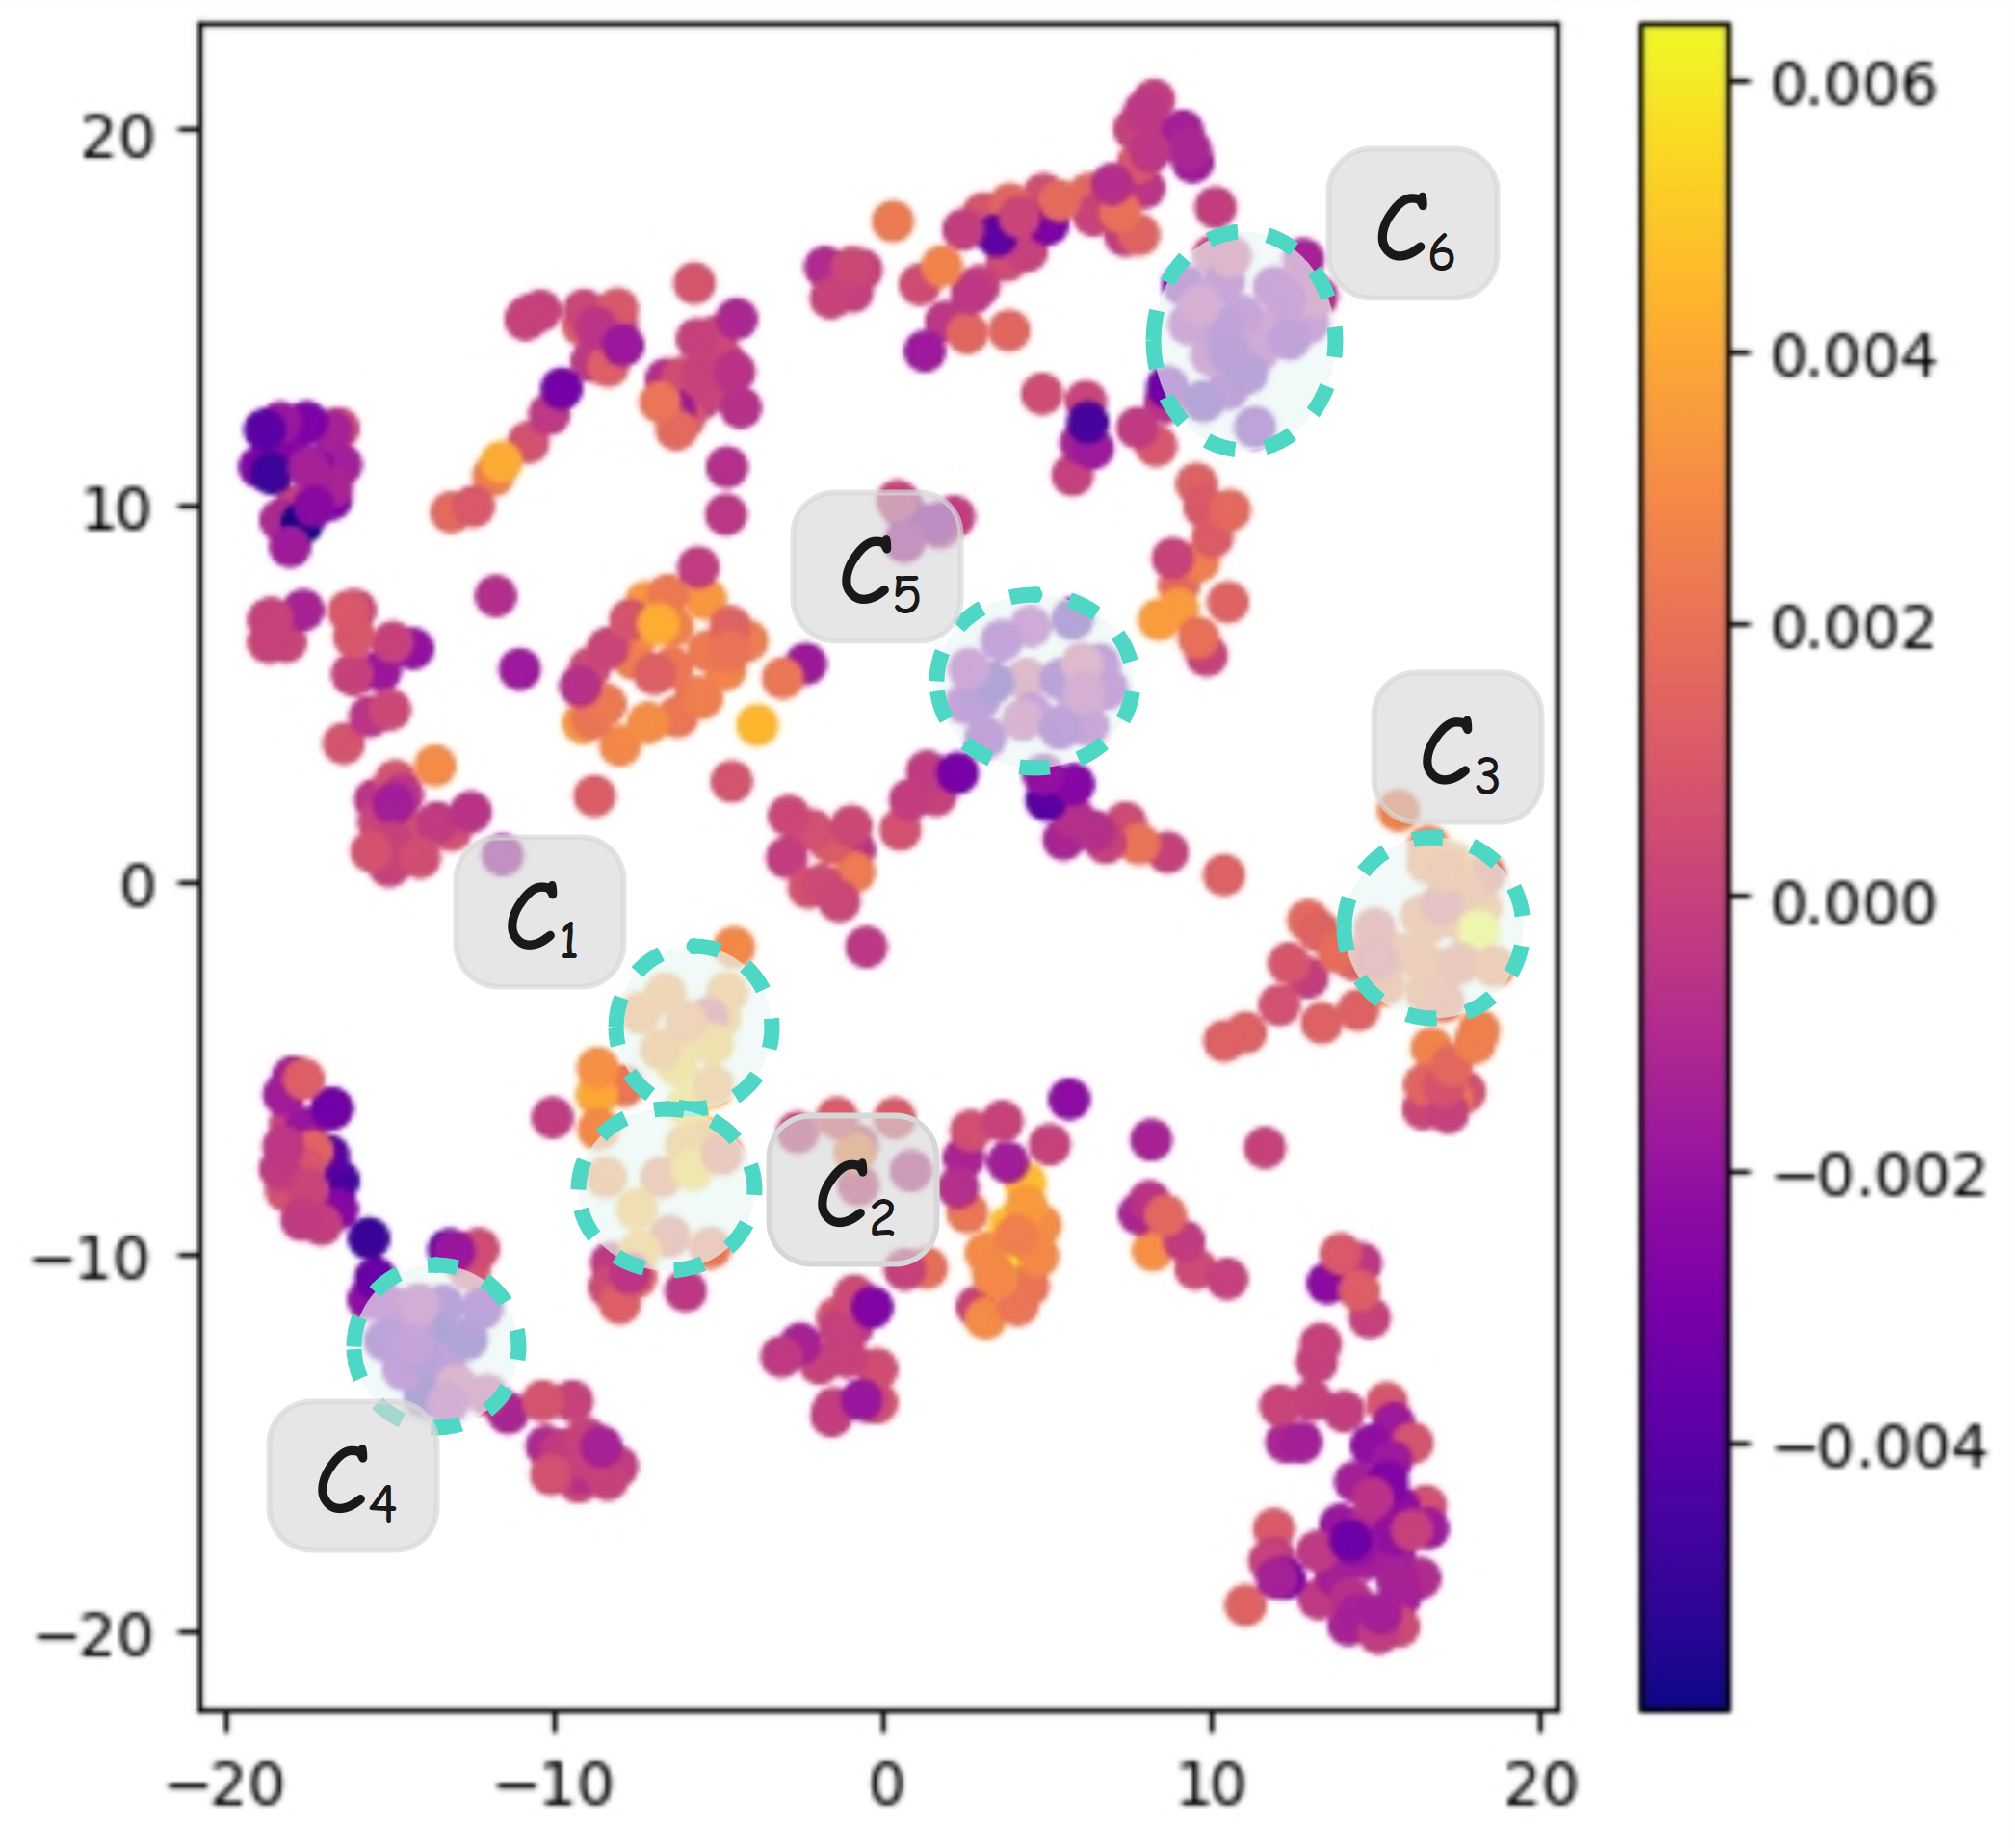
\includegraphics[scale=0.091]{intro-figure-new1.png}
    \subcaption{Influence scores of data instances}
    \label{fig1}
  \end{minipage}%
  \begin{minipage}[h]{0.5\linewidth}
    \centering
    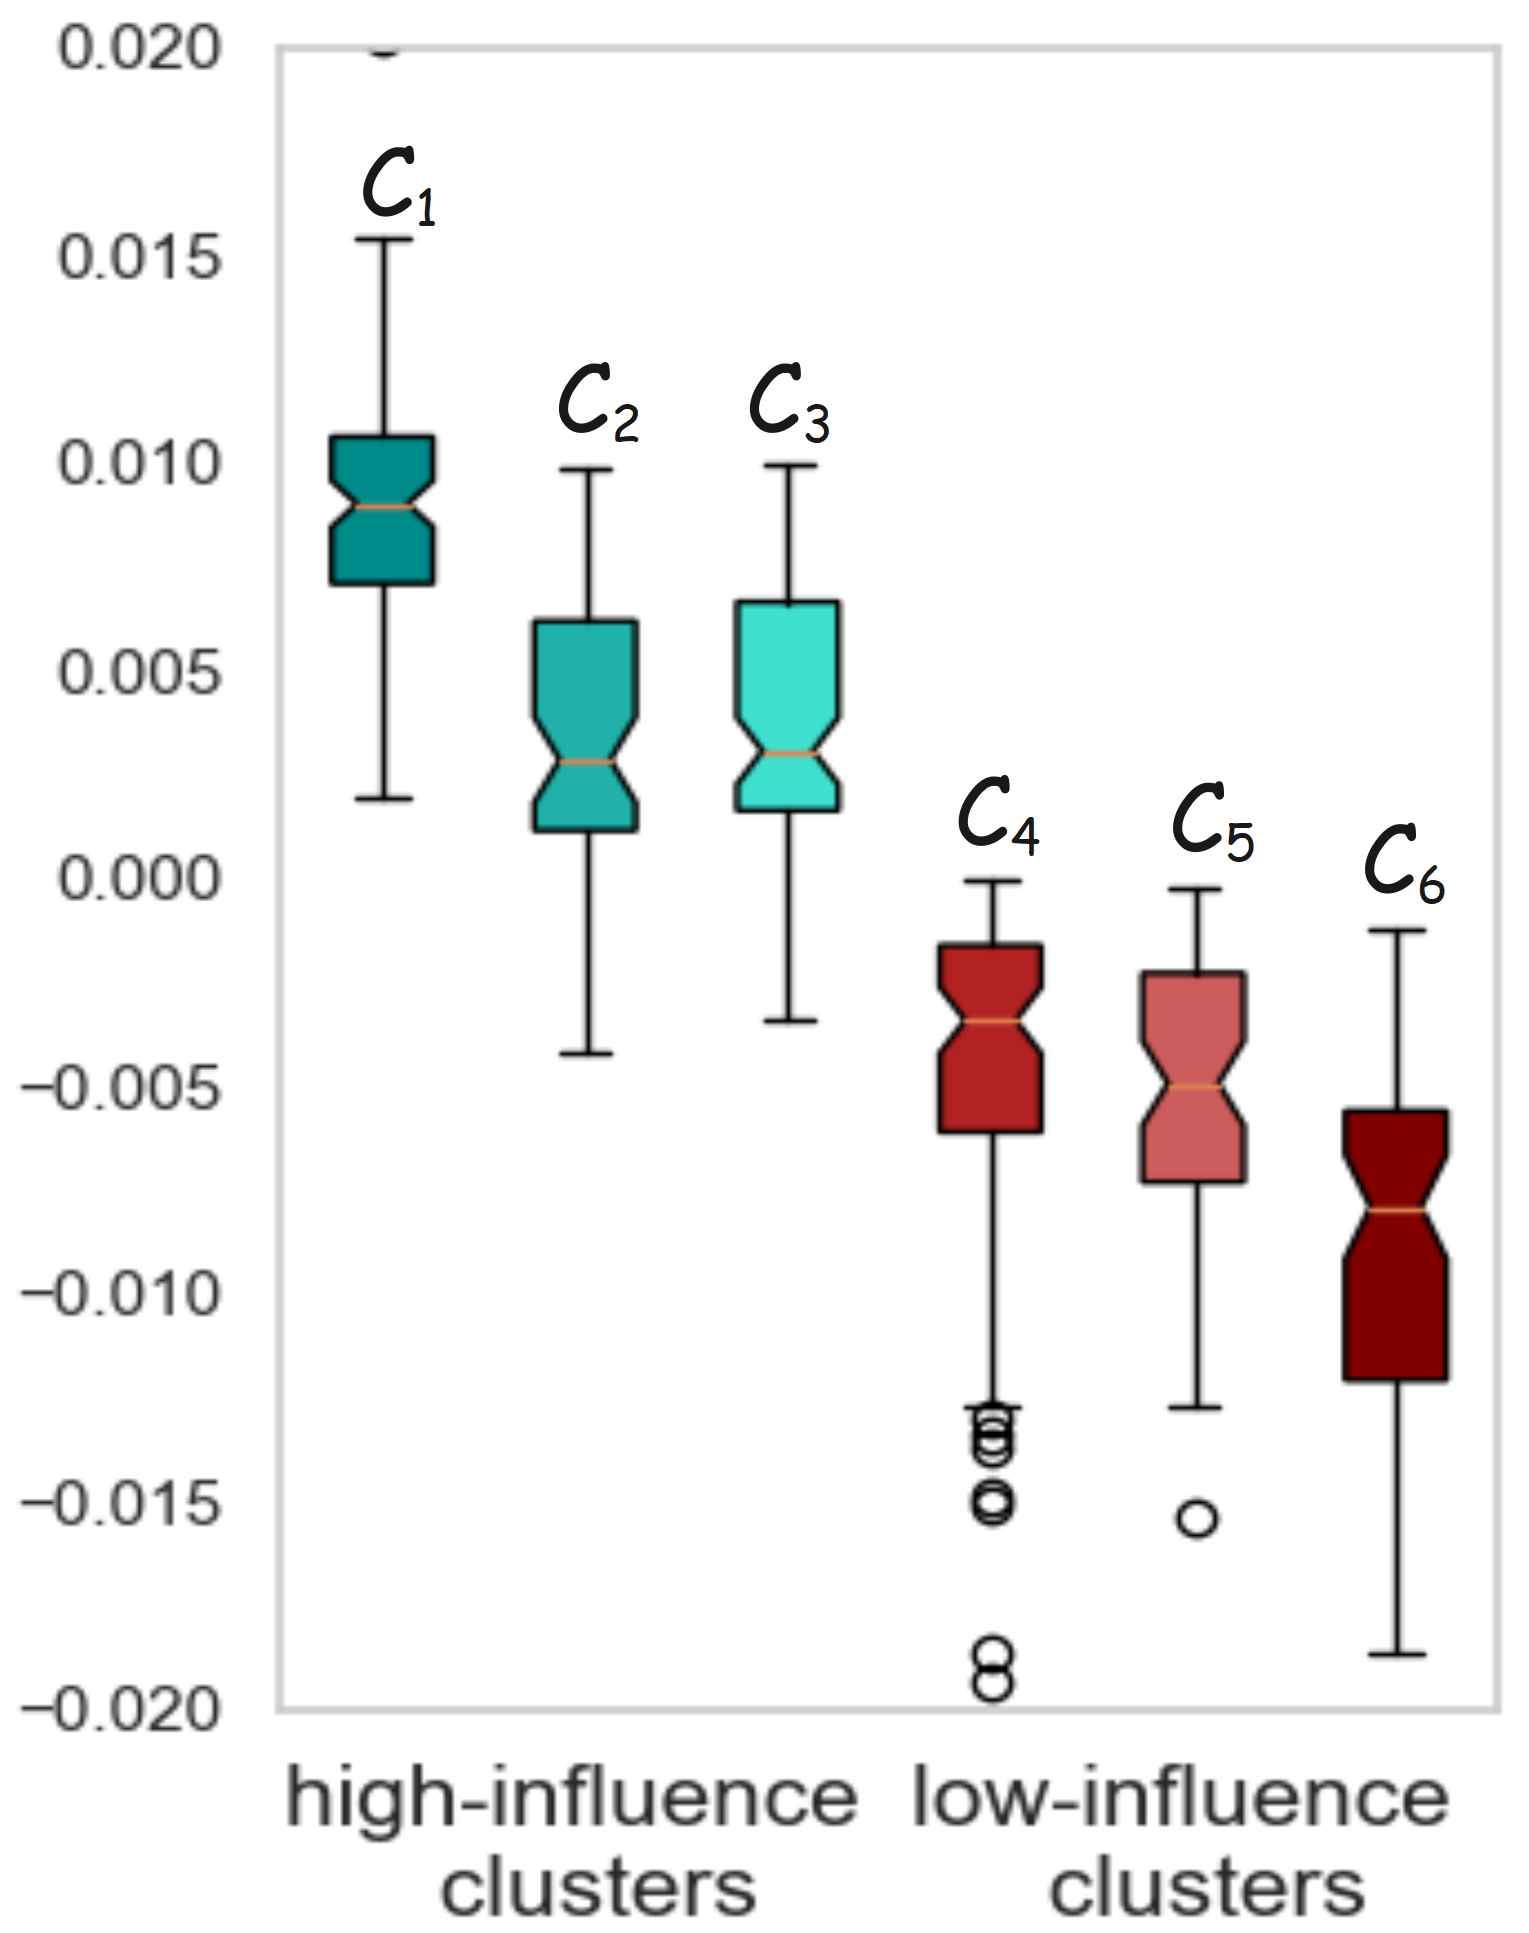
\includegraphics[scale=0.091]{intro-figure-new2.png}
    \subcaption{Influence scores in different clusters}
    \label{fig2}
  \end{minipage}
  \caption{Distribution of influence scores of some sampled data instances.}
  \label{fig:cluster_analysis}
\end{figure}

We thus propose \texttt{Quad}, a scalabe and effective data selection approach, which successfully addressing above challenges, achieves state-of-the-art pretraining results. Initially, \texttt{Quad} organizes the given dataset into clusters where the data instances within each cluster are similar, and those in different clusters exhibit diversity. Hence, we can sample a data subset from a cluster to estimate the accurate average influence of the cluster, so as to represent the cluster quality $w.r.t$ the model performance. %\lei{What do we mean by quality? If it means influence score, I won't suggest to replace it with influence score. Quality is too general and vague.}

Next, leveraging the property of the attention-based Transformer architecture which is widely adopted by the LLMs, we design a novel method to accurately compute the influence of an instance on LLM pre-training. More specifically, rather than solely relying on the MLP layers to compute the influence~\citep{koh2017understanding, yu2024mates, grosse2023studying, engstrom2024dsdm}, we incorporate the attention layers such that the influence computation considers more semantic information. In addition, given that calculating the Hessian matrix is time-consuming, particularly for attention layers with complex interactions, we incorporate the Kronecker product to approximate  the Hessian matrix, thereby greatly expediting the computation. This successfully addresses the computation cost challenge.

%Given that calculating the Hessian matrix is time-intensive, particularly for attention layers with intricate interactions, we utilize the Kronecker product to approximate the Hessian matrix, thereby speeding up the computation.
%diversity
To improve diversity, we apply the Multi-Arm Bandit (MAB) technique, where each cluster is regarded as an arm of the MAB. Upon selecting an arm, we draw samples from the cluster to calculate influence scores. Subsequently, \texttt{Quad} iteratively samples from clusters, taking into account both the influence score and data diversity, e.g., whether the cluster has already been sampled. Moreover, because this sampling strategy effectively avoids calculating the influence of all instances, it further speeds up the data selection process.

%We also extend the efficient EK-FAC method~\citep{grosse2023studying} to attention layers, which effectively mitigates the first limitation.



%%上一段中最后一个XXX的部分
% Nevertheless, in larger models, the attention layers extract deep semantic information from the data through several interacting weight matrices. This interaction challenges the assumption of layer independence, rendering the calculation of influence scores for MLP layers unsuitable. To address this, we extend the accelerated $iHVP$ computation method to attention layers, allowing more precise influence computation, which effectively mitigates the first limitation.

%zc:在~\citep{grosse2023studying}中,将EK-FAC方法应用于计算mlp层的influence function上,并取得了成功(EK-FAC is competitive with the more traditional LiSSA algorithm in the accuracy of the influence estimates, despite being significantly faster)。然而,大模型的attention层中同样梯度了数据中诸多深层的语义信息。由于attention层中的多个权重矩阵之间存在交互,因此无法简单得像mlp层那样假设不同层之间相互独立,分别计算influence得分。因此,我们将传统的EK-FAC方法扩展到了attention层中,使得用ek-fac方法计算influence更加准确。
We summarize our main contributions as follows:

\begin{itemize}

\item To balance the quality and diversity, we incorporate an iterative MAB solution to first cluster the data instances and select data instances from these clusters.

\item We propose a novel method to compute the influence function in attention-based Transformer architecture, so as to precisely measure the data quality in LLM pre-training.
%\item Experiment shows \textcolor{red}{\texttt{Quad} outperforms all current data selection strategies, achieving significantly better results than other foundational approaches, while employing minimal computational resources.}

\item Experiments on the widely-used dataset Slimpajama and 9 popular downstream tasks demonstrate that ~\texttt{Quad} significantly outperforms state-of-art data selection methods by 1.39\% in zero-shot accuracy, also with low computation resources consumption. 

\end{itemize}

%%%%%%%%%%%influence有效:
%由图1的high-score cluster/low-score cluster这三个例子中可以看出,influence可以召回和验证集很相关的数据,这时,如果我们使用高质量数据作为验证集,便可以从数据池中召回与之相似高质量的数据。

%%%%%%%%%%%influence+聚类有效:
%然而,由于再pretrain阶段数据条数过多,因此倘若一一对数据计算influence score则计算成本过高。这时,根据图2,我们发现,同一个簇中的influence得分呈现一致性(influence与数据的topic呈现正相关性)。因此,可以通过对一个簇采部分样本,计算influence score,来代表这个簇的influence得分。这时,一个最简单的方法就是:我们从每个簇中采样m条样本,分别计算每个簇的平均influence得分,并取influence平均得分最高的topk个簇来训练模型。

%%%%%%%%%%%influence+聚类+多臂老虎机有效:
%然而,在图一中可见,倘若仅选择influence score最高的topk个簇,会导致筛选出的数据分布于集中于某几个很小的区域,多样性过低,影响模型性能。这时,我们使用多臂老虎机来平衡数据的探索与利用。使最终召回的数据既有较高的质量,又有较高的多样性。



%%%%%%%%%%%%%%%%周日下午的电话讨论
% 全量数据算influence慢-->聚类-->每个簇中选部分样本来代表整个簇

%论文署名:张驰、钟老师(共一第二)、张宽、(汪老师、庄薪霖、马老师、白天一、邱老师)、(王雨卉、范老师、曹老师、曹老师学生)、(柴老师、何老师)、(袁老师、王老师)

% 提出influence
% 1. influence——>慢、多样性差——>cite图1&图2
% 2. 强调多样性的好处——>找几篇文章
% 3. 引出:多样性与influence function结合-->聚类
% 4. 想几个简单的基于聚类的baseline
% 5. 从聚类到多臂老虎机如何过渡——>和曹老师讨论topk的问题
%
%Attempts to address this show that the quality of training data is dependent on intrinsic quality and diversity. 
%
%High-quality data help models understand context and capture semantic details, while the diversity in the data ensures that the models are generalizable and applicable to different tasks.

% %%%%%%%%%%%%%%%%%%%%%%%%%%%%%%%%大模型scaling-law
% ~\citep{brown2020language} ~\citep{hoffmann2022empirical} ~\citep{touvron2023llama}

% %%%%%%%%%%%%%%%%%%%%%%%%%%%%%%%%%%%%%%%%大模型大数据量消耗更多的资源、耗时长
% ~\citep{hoffmann2022empirical} ~\citep{kaplan2020scaling} ~\citep{chowdhery2023palm} ~\citep{touvron2023llama}



% %%%%%%%%%%%%%%%%%%%%%%%%%%%%%%%%%%%%%%%%%%%%%%%%数据质量
% %MATES
% %1. 数据筛选可以提高generalization
% ~\citep{engstrom2024dsdm} ~\citep{wettig2024qurating}
% %2. 数据筛选可以提高模型的scaling efficiency
% ~\citep{biderman2023pythia}
% %3. 数据筛选可以introduce specialized capabilities
% ~\citep{lin2024rho}

% %DSIR
% %数据质量对模型的表现很重要
% ~\citep{brown2020language} ~\citep{du2022glam} ~\citep{gururangan2020don} ~\citep{hoffmann2022empirical} ~\citep{raffel2020exploring}

% %Qurating
% % right training data is essential for producing state-of-the-art large language models
% ~\citep{brown2020language} ~\citep{chowdhery2023palm} ~\citep{rae2021scaling}

% %CMU做的influence function
% %data valuation, which quantifies the contribution of each training data to the model output, has been discussed as a potential technical solution for tackling these societal issues
% ~\citep{castro2023data} ~\citep{ghorbani2019data} ~\citep{huang2023citation} ~\citep{jia2019towards} ~\citep{worledge2024unifying} ~\citep{zhao2023addressing}

% %RHO-1  
% %数据质量的重要性
% ~\citep{brown2020language} ~\citep{team2024gemma}

% %%%%%%%%%%%%%%%%%%%%%%%%%%%%%%%%%%%%%%%%%%%%%%%%%多样性
% %在去重过程中引入多样性
% ~\citep{abbas2023semdedup} ~\citep{tirumala2023d4}

% %MATES:随着训练数据的增加,基于perplexity的方法效果会变差,因为会降低数据的多样性
% ~\citep{longpre2023pretrainer}

% %多样性的重要性
% %在nlp中,when the classes of the pretraining task are sufficiently diverse, then pretraining can significantly improve the sample efficiency of downstream tasks(PMLR)
% ~\citep{zhao2023blessing}

% %We show that the diversification of training samples alleviates overfitting and improves model generalization and accuracy.(COLING)
% ~\citep{yu2022can}

% %由于pretrain阶段多样性的文章较少,因此对其它阶段进行调研:
% %在ICL(in-context learning)阶段
% %Thus, when pretrained on data with task diversity greater than the threshold, transformers can optimally solve fundamentally new tasks in-context. 
% ~\citep{raventos2024pretraining}

% %在sft阶段
% % addresses the significance of data diversity on model performance, yet neglects to maintain data diversity during selection
% ~\citep{zhou2024lima}

% % discovered that mixing training data from different tasks improves LLMs’ capabilities in low-resource scenarios
% ~\citep{dong2023abilities}

%数据多样性
\

% To obtain high-quality data, researchers initially used intuitive methods such as semantic deduplication and similarity search to enhance the quality of the data. Later, researchers used high-performance models (\textit{e.g.}, GPT-4) to score and select data based on predefined metrics. To further reduce computational costs, the researchers next trained semantic classifiers for high-quality sequence and token-level selection. Furthermore, feedback signals, such as signals like early loss, perplexity (PPL), and the influence function, were used to gauge how models perceive data, allowing model perception for better and more informed data selection.

% Considering that during the model training process, the state of the large model and its data preferences can vary depending on the pretraining data. Therefore, approaches such as Qurating~\citep{wettig2024qurating}, which use fixed metrics to assess data quality without accounting for downstream tasks and the continuously evolving state of the model, are overly heuristic.

% Thus, we use influence functions~\citep{koh2017understanding}~\citep{pruthi2020estimating}, which can capture the model's data preferences and are applicable in many domains. However, relying on them alone only favors certain data subsets, leading to reduced data diversity. To balance the model's data preferences and inherent diversity, this paper proposes a data selection strategy using reinforcement learning and influence functions.

% Like Qurating~\citep{wettig2024qurating}, we assert that using a whole ntework domain, such as Wikipedia, to proxy data quality is imprecise. Therefore, we perform clustering to determine whether high-quality data can be grouped together. In our experiments , we observed that the influence scores of the data tend to correlate positively with the topic of the data, which is consistent with intuitive expectations, which is similar to the finding of LESS~\citep{xialess}.

% To balance data quality and diversity, we treat each data cluster as an arm of a Multi-Armed Bandit (MAB) problem. We use the influence score as the reward for the MAB, thus selecting the data that most effectively enhance the performance of the large model.

% We summarize our main contributions as follows:

% 1. influence + 聚类 ——> 降低数据筛选的成本
% 2. 将近似ihvp的EK-FAC方法修改到了attention层上
% 3. 将mab应用于数据选择的框架,从而平衡数据筛选的相关性和多样性




% Papers to be submitted to ICLR 2025 must be prepared according to the
% instructions presented here.

%% Please note that we have introduced automatic line number generation
%% into the style file for \LaTeXe. This is to help reviewers
%% refer to specific lines of the paper when they make their comments. Please do
%% NOT refer to these line numbers in your paper as they will be removed from the
%% style file for the final version of accepted papers.

% Authors are required to use the ICLR \LaTeX{} style files obtainable at the
% ICLR website. Please make sure you use the current files and
% not previous versions. Tweaking the style files may be grounds for rejection.





\section{Related Work}

%%zhp(solved): related work主要介绍预训练数据筛选相关的工作和MAB就好了。
%High-quality data selection has been widely studied in large language models.

%\subsection{heuristic data selection}%基于数据本身进行筛选

\textbf{Rule-based Methods.}
Initially, researchers often relied on intuition to design hand-crafted heuristics~\citep{soldaini2024dolma} and ~\citep{penedo2023refinedweb}, aiming to improve data quality. Deduplication is another typical approach for selecting pretraining data, such as ~\citep{penedo2023refinedweb} and SemDedup ~\citep{abbas2023semdedup} which use keyword-based and semantic deduplication, respectively. Additionally, certain approaches employ $n$-gram similarity~\citep{gao2020pile, xie2023data} to assist in choosing corpora that is semantically aligned with the validation set data.
Although these methods effectively filter out noise and redundant data from web sources, they rely on simple heuristics and cannot be well generalized.

\textbf{LLM As a Selector.}
Although large models such as GPT-4 can effectively assess data quality due to their semantic comprehension capacity, the metrics utilized to rate data ($e.g.,$ writing style, educational value etc.) heavily rely on human intuition~\citep{wettig2024qurating, penedo2024fineweb, zhang2024autonomous, gunasekar2023textbooks}. This often leads to a mismatch between the selected data and the data desired by the model. 

%Although large models such as GPT-4 showcase considerable semantic comprehension and can effectively assess data quality, the metrics utilized  to rate data often rely heavily on human intuition. This reliance frequently results in a mismatch between the selected data and the data truly required by the model.


\textbf{Surrogate Models.}
DeepSeekMath ~\citep{shao2024deepseekmath} proposes an active learning strategy to train a web data classifier. Similarly, in MATES~\citep{yu2024mates}, a surrogate model was developed to estimate the influence scores of the data instances. RHO-1 ~\citep{lin2024rho} used a surrogate model trained with high-quality data to perform token-level data filtering. 
%However, these techniques usually require significant GPU resources for surrogate model training, and classifiers tend to be domain-specific, limiting their adaptability across various domains.
However, these surrogate models are not trained over large-scale data, and thus their generalizatio ability is limited.

%\subsection{model-aware data selection}%基于模型的状态进行筛选

%\textbf{Loss-based method.} In ODM ~\citep{albalak2023efficient}, the loss incurred during the pretraining phase is utilized as a  signal to dynamically adjust the data distribution throughout the training process of the model. However, \textcolor{red}{there is no clear correlation between loss and data quality, simply} employing the loss as signal \textcolor{red}{is easily affected by the anomalous data.}

%However, employing the loss as a  signal will lead to imprecise data scoring because it does not directly influence the training result like the gradient.   
%Furthermore, we argue that using an entire domain, such as Wikipedia, as a proxy for data quality is inherently imprecise.

%在mates中,通过使用early loss近似influence function来估计每个数据点对模型的影响
\textbf{Perplexity} serves as a metric for selecting high-probability data in a language model. In ~\citep{chen2024towards, marion2023less, muennighoff2024scaling, wenzek2019ccnet}, perplexity (PPL) is utilized to filter data. As also discussed in Qurating~\citep{wettig2024qurating}, we observe that this method often incorporates a significant amount of simple and redundant data, because they are easy for the model to predict.

\textbf{Influence Function} 
~\citep{grosse2023studying, choe2024your} demonstrates that influence function can reveal the impact of training data on the performance of large models. Consequently, LESS~\citep{xialess} and MATES ~\citep{yu2024mates} utilize influence functions for selecting data during the SFT and pretraining phases, respectively. For large models, computing influence functions is computationally expensive. ~\citep{grosse2023studying}. Hence, given the large amount of data handled during pretraining, directly using LESS~\citep{xialess} for data selection at this stage poses considerable difficulties. To overcome this, MATES~\citep{yu2024mates} employs a proxy model to approximate the influence score across the full dataset. 
However, the limited capacity of this small proxy model hinders its ability to provide accurate influence scores.
%
Furthermore, relying on the influence to select data solely often leads to a lack of diversity in the chosen data. %Therefore, both MATES~\citep{yu2024mates} and Qurating~\citep{wettig2024qurating} use heuristic methods, such as Gumbel sampling, to ensure a balance between diversity and quality.

% \textbf{Multi-Armed Bandit}
% Multi-armed bandit algorithms~\citep{vermorel2005multi} represent a simple yet effective approach in reinforcement learning. 
% In ODM ~\citep{albalak2023efficient}, the loss incurred during the pretraining phase is utilized as a reward signal to dynamically adjust the data distribution throughout the training process of the model. However, employing the loss as a reward signal in this approach will lead to imprecise data scoring. Furthermore, we argue that using an entire domain, such as Wikipedia, as a proxy for data quality is inherently imprecise. Also, ~\citep{albalak2024improving} employs gradient similarity as a reward signal in a Multi-Armed Bandit framework to filter auxiliary data for few-shot learning. However, this approach does not account for the interrelationships among auxiliary datasets. Furthermore, due to the substantially larger volume of data in the pretraining phase compared to that in few-shot learning, it is challenging to compute gradient similarities for all data points and to update the large model in real time. In contrast, the influence function can better account for the state of the model.
% 1. Data annealing
% Data annealing作为有效的模型训练方法[1][29],需要在训练的后期使用高质量的数据。因此,During the data annealing process, it is key to explore various potential strategies for data collection. 然而,现阶段data annealing的通常使用人为设计的filter[1]来获得高质量数据,较为heuristic。
% 2. 基于数据本身进行筛选
%   1. Manual intuition
%     1. 在早期,人们往往根据直觉,设计hand-crafted heuristics,如[26]、[27]来提高数据质量。deduplication是pretrain数据筛选过程中的另一个standard approach,如[27]、semdedup[16]分别通过关键词和语义去重。尽管这些方法可以有效过滤掉网页数据中的噪音、冗余数据,但是人们需要更精确的方法来寻找候选数据池中的desirable examples。
%   2. GPT大模型
%     1. 尽管GPT般大模型具备卓越的语义提取能力,能够分析数据的语义信息。但GPT对数据进行打分的指标往往过于依赖人们的直觉,较为heuristic,这与模型真实需要的数据往往存在一定偏差。其中,较为代表的工作包括qurating[6],Finweb[19], autoDS[20], [34]
%   3. 代理模型
%     1. deepseekmath[4]中,通过active learning方式训练了一个网页数据分类器。MATES[5]中,训练了代理模型来估计数据样本的infleunce score。RHO-1[24]中使用高质量数据训练出的代理模型来从token级别进行数据筛选。然而,在这些方法中,所训练的小模型往往都需要耗费大量的GPU资源,且分类器仅能针对某一特定领域,难以做到多领域通用。
% 3. 基于模型状态进行筛选
%   1. perplexity filtering:[2][21][31][33]中使用ppl作为过滤数据的指标。然而,我们发现这样会包括很多简单且重复的数据,因为这对模型来说很容易预测。
%   2. Early loss: [30]
%   3. 基于KL散度的方法——GIO[17],基于N-gram的方法——DSIR[14],难以发现数据之间的深层联系,在下游评测集中表现较差。
%   4. Influence function:[7][18]发现可以通过influence来揭示训练数据对大模型效果的影响。此后,LESS[13]和MATES[5]分别将influence用在了sft和pretrain阶段的数据筛选中。在大模型的场景下,影响函数十分消耗计算资源[7],在LESS[13]、[32]的研究中,发现first-order influence approximations are effective for data selection。同时,考虑到预训练阶段数据量过大,因此难以将LESS[13]的方法直接迁移到预训练阶段的数据筛选中。为此,MATES[5]训练了proxy model来估计全量数据的infleunce score. 然而,由于代理模型参数量较小,难以提取出数据的深层信息,导致估计influence的结果不准。同时,仅依靠influence进行数据筛选往往会导致选出的数据较为单一,因此在MATES[5]和Qurating[6]中,采用较为heuristic的gumble sampling to balance diversity and quality
% 5. 强化学习
%   1. 多臂老虎机[10]是强化学习中simple yet effiective的方法,在ODM[22]中以pretrain阶段的loss作为reward,在线动态调整预训练模型训练过程中的数据配比。然而, 在这一方法中,每次用loss作为reward,对数据的打分依然不够精确。同时,We argue that an entire domain such as Wikipedia is an imprecise proxy for data quality.
%   2. Most similar to our work, [40]使用梯度相似度作为多臂老虎机的奖励,在few-shot learning中筛选auxiliary data.然而,在这一方法中,没有考虑到auxiliary datasets之间的联系。此外,由于预训练阶段的数据量远大于few-shot learning中的数据量,因此难以对所有数据计算梯度相似度,并实时更新大模型。同时,相较于梯度相似度,infleunce function可以更好地考虑模型的状态。

% [1] Does your data spark joy? Performance gains from domain upsampling at the end of training
% [2] Towards Effective and Efficient Continual pretraining of Large Language Models
% [3] Overcoming Catastrophic Forgetting in Massively Multilingual Continual Learning
% [4] DeepSeekMath: Pushing the Limits of Mathematical Reasoning in Open Language Models
% [5] MATES : Model-Aware Data Selection for Efficient Pretraining with Data Influence Models
% [6] QuRating: Selecting High-Quality Data for Training Language Models
% [7] Studying Large Language Model Generalization with Influence Functions
% [8] Influence Selection for Active Learning
% [9] Understanding Black-box Predictions via Influence Functions
% [10] Multi-armed Bandit Algorithms and Empirical Evaluation
% [11] Sample surveys: design, methods and applications.
% [12] If Influence Functions are the Answer, Then What is the Question?(如果最终用一阶influence的话,则删掉)
% [13] LESS: Selecting Influential Data for Targeted Instruction Tuning
% [14] Data Selection for Language Models via Importance Resampling
% [15] Towards Effective and Efficient Continual pretraining of Large Language Models
% [16] SemDeDup: Data-efficient learning at web-scale through semantic deduplication
% [17] GIO: Gradient Information Optimization for Training Dataset Selection
% [18] What is Your Data Worth to GPT?LLM-Scale Data Valuation with Influence Functions
% [19] The FineWeb Datasets: Decanting the Web for the Finest Text Data at Scale
% [20] Autonomous Data Selection with Language Models for Mathematical Texts
% [21] When Less is More: Investigating Data Pruning for Pretraining LLMs at Scale
% [22] Efficient Online Data Mixing For Language Model pretraining
% [23] DoReMi: Optimizing Data Mixtures Speeds Up Language Model Pretraining
% [24] RHO-1: Not All Tokens Are What You Need
% [25] slimpajama: https://cerebras.ai/blog/slimpajama-a-627b-token-cleaned-and-deduplicated-version-of-redpajama url: https://huggingface.co/datasets/cerebras/SlimPajama-627B
% [26] Dolma: an Open Corpus of Three Trillion Tokens for Language Model Pretraining Research
% [27] The refinedweb dataset for falcon LLM: Outperforming curated corpora with web data only.
% [28] Deduplicating Training Data Makes Language Models Better
% [29] The Llama 3 Herd of Models
% [30] Rethinking Optimization and Architecture for Tiny Language Models
% [31] Scaling data-constrained language models
% [32] Estimating Training Data Influence by Tracing Gradient Descent
% [33] When Less is More: Investigating Data Pruning for Pretraining LLMs at Scale
% [34] Textbooks are all you need
% [35] Optimizing data usage via differentiable rewards
% [36] An empirical analysis of computeoptimal large language model training
% [37] Enhanced transformer with rotary position embedding
% [38] Llama: Open and efficient foundation language models
% [39] Perplexed by Perplexity: Perplexity-Based Pruning with Small Reference Models
% [40] Improving Few-Shot Generalization by Exploring and Exploiting Auxiliary Data

\section{Methods}
First, we present our problem statement in \S \ref{sec:framwork}. Next, in \S \ref{sec:mab}, we explain how our method achieves the  balance between quality and diversity in selecting pretraining data. Finally, in \S \ref{sec:ek-fac}, we 
introduce how we compute the influence with attention layers more accurately and efficiently.

%describe the enhancements made for computing influence accuracy.
% \begin{itemize}
% \item Initially, we present our problem statement in \S \ref{sec:framwork}.
% \item Next, in \S \ref{sec:mab}, we explain how our method strikes a balance between quality and diversity in selecting pretraining data.
% \item Finally, in \S \ref{sec:ek-fac}, we describe the enhancements made for computing influence accuracy.
% \end{itemize}
\begin{figure}[h]
\begin{center}
%\framebox[4.0in]{$\;$}
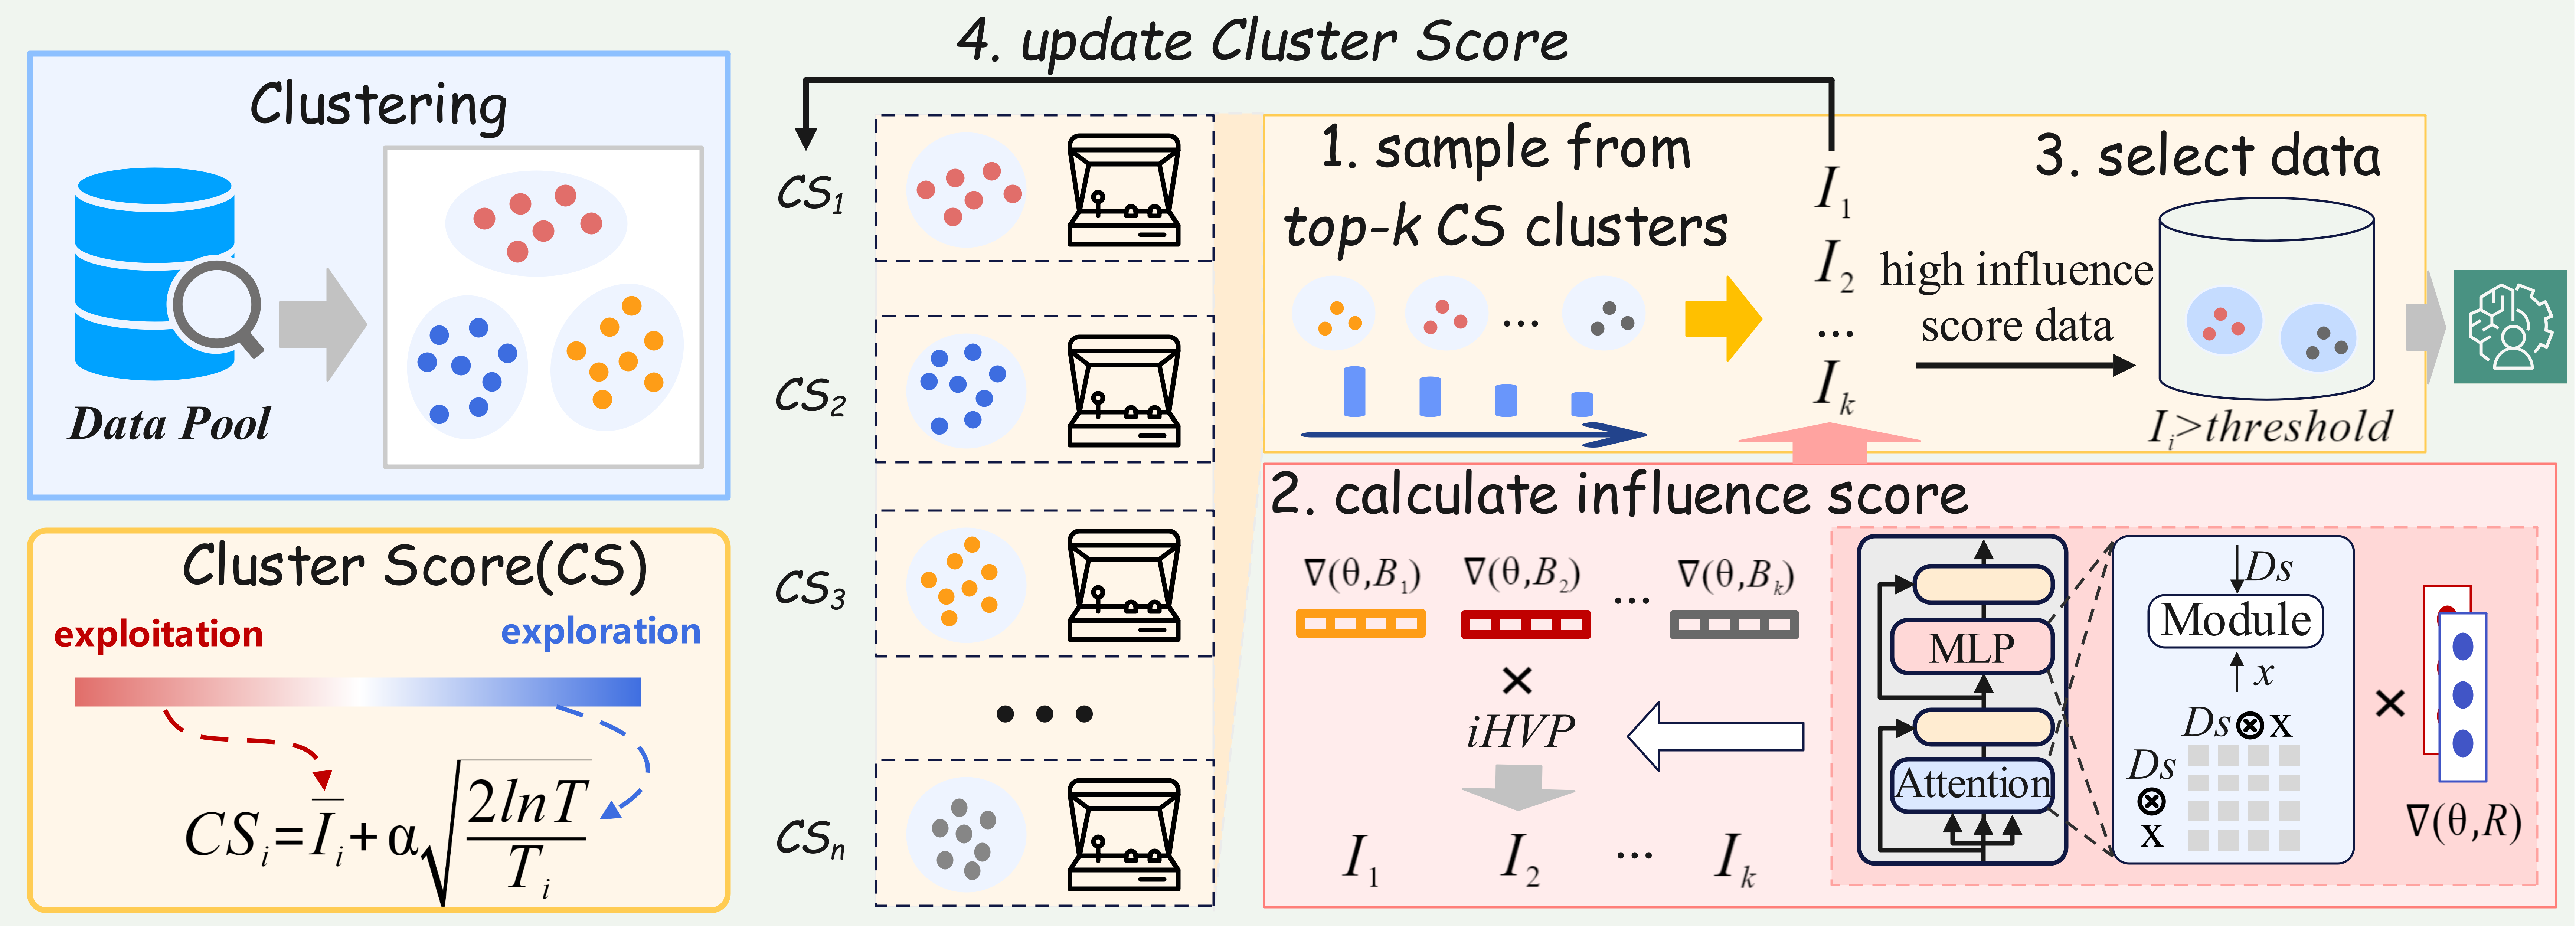
\includegraphics[width=1\textwidth]{mab-new.png}
\end{center}
\caption{Overview of \texttt{Quad}}
\label{fig3}
%\vspace{0.5cm}  % 调整图片标题与说明之间的间距
  
  \begin{minipage}{1\textwidth}
    \small  % 将文字缩小,可以根据需要调整大小
    %Figure~\ref{fig2} shows that the combined data reveals a notable uniformity in the influence distribution. Hence, we utilize a recognized pretrained embedding model to execute k-means clustering on the data from the candidate pool.
  \end{minipage}
\end{figure}
% \label{headings}

%%zhp(solved): 章节之间可以参考mates之类的论文,加一些过渡的语句,比如in this section, we will introduce our proposed method...

%%zhp(solved,删除了所有包含batch的字眼): 这里不要叫a batch of data,大家看到batch都会认为是deep learning里面的batch,可以换成比如a subset of data


\subsection{Problem Definition}
\label{sec:framwork}
To enhance the capabilities of large models, it is necessary to retrieve relevant data from a large pool of candidate data and perform further training for the large model. 
%
Formally, given the pool $D_c$ and a reference set $D_r$, our problem is to select a subset  $D_b \subset D_c$  to fine-tune the large model $M$, with the aim of minimizing the loss of the updated model $M'$ in the reference set $D_r$. 


%%zhp(solved): 先放方法的架构图,再介绍每个模块,伪代码可以等到方法都介绍完了之后,再贴
%zc:这个approach的整体流程如图2所示,我们的方法可以分为以下4步:首先,我们从Cluster Score(CS)得分最高的$top-k$个簇中采样;分别对这些样本计算influence得分;这时,我们选出大于阈值的top score data,并利用计算出的influence得分更新每个簇的cluster score(CS)

%%zhp(solved): 这些小节对应咱们的子模块,然后都换成我们的叫法,不要直接叫MAB这些,要不然别人就会觉得都是别人的方法

\subsection{balance between quality and diversity}~\label{sec:mab}
%As shown in Figure~\ref{fig2}, there are significant variations in the distribution of influence scores among different clusters. Meanwhile, within each cluster, the influence values also exhibit fluctuations around the average, suggesting some degree of uncertainty. 
As shown in Figure~\ref{fig2}, there are significant variations in the distribution of influence scores among different clusters.
To achieve the quality-diversity balance, it is necessary to know the precise average influence score for instances in each cluster.
However, Figure~\ref{fig2} shows that the influence scores for each cluster also fluctuate around the average, indicating a certain level of uncertainty. Estimating the average with a small sample size will not be accurate enough, while taking a large number of samples to compute the average influence is costly.
%
%However, Figure~\ref{fig2} shows that the influence values for each cluster also fluctuate around the mean, indicating a certain level of uncertainty. Estimating the mean with a small sample size will lack accuracy, while taking a large number of samples is costly.

Hence, we propose to use the MAB~\citep{vermorel2005multi} technique that is capable of making decisions iteratively under uncertainty. At a high level, each cluster represents an arm of the MAB, and during each iteration, a cluster with a high average influence score tends to be selected and sampled. We will then compute the influence of data instances to update the average. Moreover, clusters that are not visited often present significant opportunities for sampling to balance the diversity.


%a subset of data $B_i$ will be  sampled from the respective cluster to calculate influence scores.


%It considers N possible actions to choose from; pulling each possible action is also known as an arm. It models an agent that simultaneously attempts to acquire new knowledge($i.e.$ exploration) and optimize their decisions based on existing knowledge($i.e.$, exploitation). The agent attempts to balance these competing tasks to maximize their total values over the period of time considered. Here, each cluster represents an arm of the MAB, and during each iteration, a subset of data $B_i$ is sampled from the respective cluster to calculate influence score, as the reward of this action.

The overall process of this approach is illustrated in Figure~\ref{fig3}. Specifically, our method can be divided into the following four steps: First, we \textit{sample the top-$k$ clusters} with the highest cluster scores (denoted by CS) computed by MAB. 
Here, the cluster score is determined by both the influence score and the sample frequency.
Then we \textit{calculate the influence scores} for the samples in each cluster (Section 3.3). At this point, we \textit{select  high scoring samples} to be added for training and use their scores to \textit{update the cluster score} for each cluster.
%
Throughout the iterative process, the MAB algorithm focuses on frequently sampling high-quality clusters that have high influence scores, which also  enhances the accuracy of their quality estimation ($i.e.,$ updating the average influence $\overline{I}_i$). Simultaneously, it ensures diversity by also sampling less-visited clusters.
Next, we discuss how to compute and update the cluster score in details.

%Throughout the iterative process, the MAB algorithm focuses on frequently sampling high-quality clusters that have substantial influence scores, thereby enhancing the precision of their quality estimation (i.e., average influence). Simultaneously, it ensures diversity by occasionally sampling less-visited clusters.

%Conversely, it also performs diverse sampling on low-scoring clusters during exploration period and rarely revisits them later, which greatly accelerates and benefit the data selection process.

%从figure 2中,我们发现, 同一个簇中数据的influence值往往围绕着平均值上下波动,具有一定的uncertainty;与此同时,不同簇数据influence的分布存在着明显的差异.
%%zhp(solved): 这个图片更像是方法的流程图,如果要放的话,就换成英文版本,放在第三章的一开始吧。否则这里更应该画方法的架构图,把我们的方法分成几个子模块,然后子模块跟小节的标题尽量对齐。
%zc:这里应该有个同学帮忙重新画了,应该明晚画完

%%zhp(solved): 这个offline的模块就不要放在这里讲了,在第三章一开始流程图的下面,就直接讲:正如我们introduction介绍的,聚类后的数据在influence分布上有很强的一致性,因此我们采用别人预训练的embedding模型,对预训练数据做kmeans聚类。
%%zhp(solved): 我们用的不是word embedding模型!!!

%%zhp(solved): 这里都没有做实验,怎么能讲experiments have shown。你应该是说正如我们introduction里面的那个统计分布图,发现相邻簇的内容和influence都有很大的相似性,如果只依赖influence score对簇进行采样,数据的多样性就会很差,所以我们就根据簇之间的距离/相似度,对比较相似的簇做降权。
%zc:这里的逻辑有点奇怪,'如果只依赖influence score对簇进行采样,数据的多样性就会很差‘这句话和前后好像因果关系不是很强
\textbf{Cluster Score (CS).} The Upper Confidence Bound can effectively balance exploration ($i.e.,$ data diversity) and exploitation ($i.e.,$ data quality), so we use it as the cluster score to evaluate each cluster, as shown in Equation (1). 
%
Specifically, the cluster score is determined by the average influence score $\bar{I_i}$ and the exploration score $\sqrt{\frac{2\ln {\sum_j{T(C_j)}}}{T(C_i)}}$, where $T(C_i)$ denotes the frequency of instances sampled from cluster $C_i$, and $\sum_j T(C_j)$ denotes  the total times of samples taken from all clusters.
%In particular, the cluster score is computed based on the mean influence score $\bar{I_i}$ and the exploration score $\sqrt{\frac{2\ln {\sum{T(C_j)}}}{T(C_i)}}$, where $T(C_i)$ represents the frequency of instances taken from cluster $C_i$, and $\sum T(C_j)$ signifies the total count of samples taken from all clusters.

\begin{equation}
    CS_{i}=\bar{I_i}+\alpha\sqrt{\frac{2\ln {\sum_j{T(C_j)}}}{T(C_i)}}
\end{equation}

\textbf{Update the cluster score.} During each iteration, a subset of data $B_i$ is sampled from each cluster with a high cluster score (CS). 
The sum of their influence score $I_i$ can be used to denote the impact of the samples from the cluster $C_i$ on the model.

%\textbf{Data selection.} 

%Spread reward to neighbour clusters
% Figure~\ref{fig1} shows that adjacent clusters have similar influence scores. Furthermore, selecting clusters purely based on influence scores can reduce data diversity. Hence, we adjust the cluster rewards by incorporating their proximity and resemblance to neighboring clusters before distributing the modified rewards. Specifically, let $N(C_i)$ denote the neighboring clusters of $C_i$, including all clusters within a distance of $\tau$ from $C_i$. Then, when a cluster $C_j$ is selected or receives a reward as a neighboring cluster:


%%zhp: 这里的+=号怎么这么奇怪,你看看latex里面是怎么写这个的
\begin{equation}
    R(C_i) += \sum_{z \in B_i}I_\theta(D_r,z)  , \quad T(C_i) += 1
\end{equation}

where $R(C_j)$ denotes the total reward accumulated by cluster $C_i$ over several iterations.%., where $T(C_j)$ denotes the number of times the current cluster has been rewarded.
Then the average influence score $\bar{I_{i}}$ for cluster $C_i$ can be represented as
    $\bar{I_i} = \frac{R(C_i)}{T(C_i)}$.
As the sample size grows, $\bar{I_i}$ for each cluster $C_i$ steadily approaches the exact average influence of the cluster, which can be used to update the cluster scores for all clusters.

\textbf{Data selection.} During each iteration, we pick a small proportion($\gamma$) of data instances from selected clusters. We also require that these instances have influence scores higher than the threshold $\tau$, otherwise we will not select them, which are then added into the training dataset.

%a small porportion


%As the sample size grows, $\bar{I_i}$ for each cluster $C_i$ steadily approaches the \textcolor{red}{exact} value of the cluster.

\begin{algorithm}[h]
    \caption{\texttt{Quad} Algorithm}
    \KwIn{Candidate data pool $D_c$, reference set $D_r$, the model $\theta$}
    \KwOut{Selected data $D_b$}
    $\mathcal{C}$ = Cluster($D_c$)\;
    \While{}{
        $C_{top\_k}$ = top-$k$ clusters with the highest Cluster Score(CS) \;

        $B_{top\_k}$ = mini-batchs sampled from $C_{top\_k}$
            
        \For{$C_i$ in $C_{top\_k}$}{      
                \quad $R(C_j)$ += $\sum_{z \in B_i}I_\theta(D_r,z),$\quad $T$($C_j$) += 1 \;                
        }
        \For{ $C_i$ in $\mathcal{C}$}{
            $\bar{I_i} = \frac{R(C_i)}{T(C_i)}$ \;
            \textbf{if} $\bar{I_i} > threshold$ \textbf{then} $D_b += \gamma C_i$\;
        }
        $CS_{i}=\bar{I_i}+\alpha\sqrt{\frac{2\ln {\sum_j{T(C_j)}}}{T(C_i)}}$ \;
    }
    \Return{$D_b$}\;
\end{algorithm}
\subsection{Influence Calculation with attention layers}
\label{sec:ek-fac}
Instead of retraining the large model with each data sample $z$, the impact of  $z$ on the model $M$ can be estimated by calculating the influence function for each instance. In this section, we extend the influence calculation to multi-head attention layers and provide acceleration techniques.
% To assess the impact of each data sample on the model, one could retrain the large model with each data sample $z$ from $D_b$. However, this approach is computationally prohibitive. Instead, the impact of each data sample point $z$ on the model $M$ can be estimated by calculating the influence function for each sample point .

% Typically, each attention layer includes the query, key, value and output layer and suppose that they are denoted by $\theta_1, \theta_2, \theta_3, \theta_4$ respectively, and the influence function can be expressed as:
\begin{equation}
    I_\theta(D_r,z)=-\nabla L(\theta,D_r)(H + \lambda I)^{-1}\nabla L(\theta,z)
\end{equation}



%Given the mutual influence among the query, key, and value layers, it is necessary to compute the Hessian matrix for the entire QKV (query-key-value) structure.
% \begin{center}
%     $I_\theta(D_r, z) = I_{\theta_1, \theta_2, \theta_3}(D_r, z) = \nabla L(\theta_1, \theta_2, \theta_3, D_r) H_{\theta_1, \theta_2, \theta_3} \nabla L(\theta_1, \theta_2, \theta_3, z)$
% \end{center}
% \begin{center}
%     $ = (\frac{\partial L}{\partial \theta_1} +\frac{\partial L}{\partial \theta_2} + \frac{\partial L}{\partial \theta_3})(H_{\theta_1} + H_{\theta_2} + H_{\theta_3} + 2\frac{\partial^2 L}{\partial \theta_1 \partial \theta_2} + 2\frac{\partial^2 L}{\partial \theta_1 \partial \theta_3} + 2\frac{\partial^2 L}{\partial \theta_2 \partial \theta_3})(\frac{\partial L}{\partial \theta_1} +\frac{\partial L}{\partial \theta_2} + \frac{\partial L}{\partial \theta_3})$
% \end{center}


% In the layers of MLP, the parameters $\theta_1$, $\theta_2$, and $\theta_3$ are mutually independent. During the process of gradient computation and update, there are usually only minimal direct dependencies between the gradients of different layers. This is particularly evident during back propagation, where the weight updates for each layer are primarily influenced by the parameters of that specific layer. 
%

% zk:θ这个参数没有进行解释,θ是大模型的参数。是否需要简单介绍H的计算公式?对于H,在lesswrong里,是这样描述的:For simplicity, as in the paper, we'll denote ∇^2_θ(1/N ∑L(z_i,θ^∗)+ϵL(z_m,θ^∗)) as H.

In the above equation, $I_\theta(D_r,z)$ denote the influence function of data $z$ on model $\theta$. $\nabla L(\theta,D_r)$ and $\nabla L(\theta,z)$ denote the gradient of reference dataset $D_r$ and data $z$, respectively. Since the training of the large model  does not often fully converge, resulting in a non-invertible Hessian matrix $H$, a regularization term $\lambda I$ is introduced~\citep{bae2022if}. Equation (3) is typically divided into the following two stages to speed up the computation:

1. Approximate the multiplication of the gradient of the validation set $\nabla L(\theta,D_r)$ and the inverse Hessian matrix $H^{-1}$  using the inverse Hessian vector product (iHVP).

2. Compute the dot product between the iHVP and the gradient of each training data point $\nabla L(\theta,z)$.

While this framework can accelerate the computation of the influence function, scaling it up to large language models (LLMs) with massive parameters is still expensive. Hence, K-FAC~\citep{martens2015optimizing, ueno2020rich} can be used to accelerate the iHVP computation by using the Kronecker product to decompose the Hessian matrix.
%In this approach, the weight matrices of each MLP layer are treated as independent, and the K-FAC method is used to approximate iHVP for each weight matrix separately.

% However, in multi-head attention mechanisms, it is challenging to assume that the weight matrices of each layer are independent, as is done with In MLP layers:
The K-FAC approximate the parameters of different MLP layer $\theta_1$, $\theta_2$ and $\theta_3$ as independent. That's because, during the gradient computation and update process, there are usually only minimal direct dependencies between the gradients of different MLP layers. This is particularly evident during back propagation, where the weight updates for each MLP layer are primarily influenced by the parameters of that specific layer. Therefore, the influence function $I_{\theta_1, \theta_2, \theta_3}(D_r, z)$ in K-FAC method can be expressed as:

\begin{equation}
    I_{\theta_1, \theta_2, \theta_3}(D_r, z) = I_{\theta_1}(D_r, z) + I_{\theta_2}(D_r, z) + I_{\theta_3}(D_r, z)
\end{equation}

% \begin{center}
%     $I_\theta(D_r, z) = I_{\theta_1, \theta_2, \theta_3}(D_r, z) = \nabla L(\theta_1, \theta_2, \theta_3, D_r) H_{\theta_1, \theta_2, \theta_3} \nabla L(\theta_1, \theta_2, \theta_3, z)$
% \end{center}
% \begin{center}
%     $ = (\frac{\partial L}{\partial \theta_1} +\frac{\partial L}{\partial \theta_2} + \frac{\partial L}{\partial \theta_3})(H_{\theta_1} + H_{\theta_2} + H_{\theta_3} + 2\frac{\partial^2 L}{\partial \theta_1 \partial \theta_2} + 2\frac{\partial^2 L}{\partial \theta_1 \partial \theta_3} + 2\frac{\partial^2 L}{\partial \theta_2 \partial \theta_3})(\frac{\partial L}{\partial \theta_1} +\frac{\partial L}{\partial \theta_2} + \frac{\partial L}{\partial \theta_3})$
% \end{center}

In attention mechanisms, there exist complex connections between the Query, Key, and Value layers. As the right-upper corner of Figure~\ref{multi-head-attention} shows, separately calculate the hessian matrix of Query, Key and Value layers, will miss massive information of 
%exemplified by parameters like $\frac{\partial^2 L}{\partial \theta_1 \partial \theta_2}$, $\frac{\partial^2 L}{\partial \theta_1 \partial \theta_3}$, and $\frac{\partial^2 L}{\partial \theta_2 \partial \theta_3}$. 
Consequently, it is essential to consider the QKV layers as a unified layer $\theta_{qkv}$ when computing the influence function. Therefore, the influence function $I_{\theta_{att}}(D_r, z)$ can be expressed as:
\begin{equation}
I_{\theta_{att}}(D_r, z) = I_{\theta_{qkv}}(D_r, z) + I_{\theta_{o}}(D_r, z)
%$I_{att}(D_r, z) = \nabla L(\theta_{qkv}, D_r) H_{\theta_{qkv}}^{-1} \nabla L(\theta_{qkv}, z) +\nabla L(\theta_{o}, D_r) H_{\theta_{o}}^{-1} \nabla L(\theta_{o}, z)$
\end{equation}

% Typically, each attention layer includes the query, key, value and output layer and suppose that they are denoted by $\theta_1, \theta_2, \theta_3, \theta_4$ respectively, and the influence function can be expressed as:

\begin{figure}[h]
\begin{center}
%\framebox[4.0in]{$\;$}
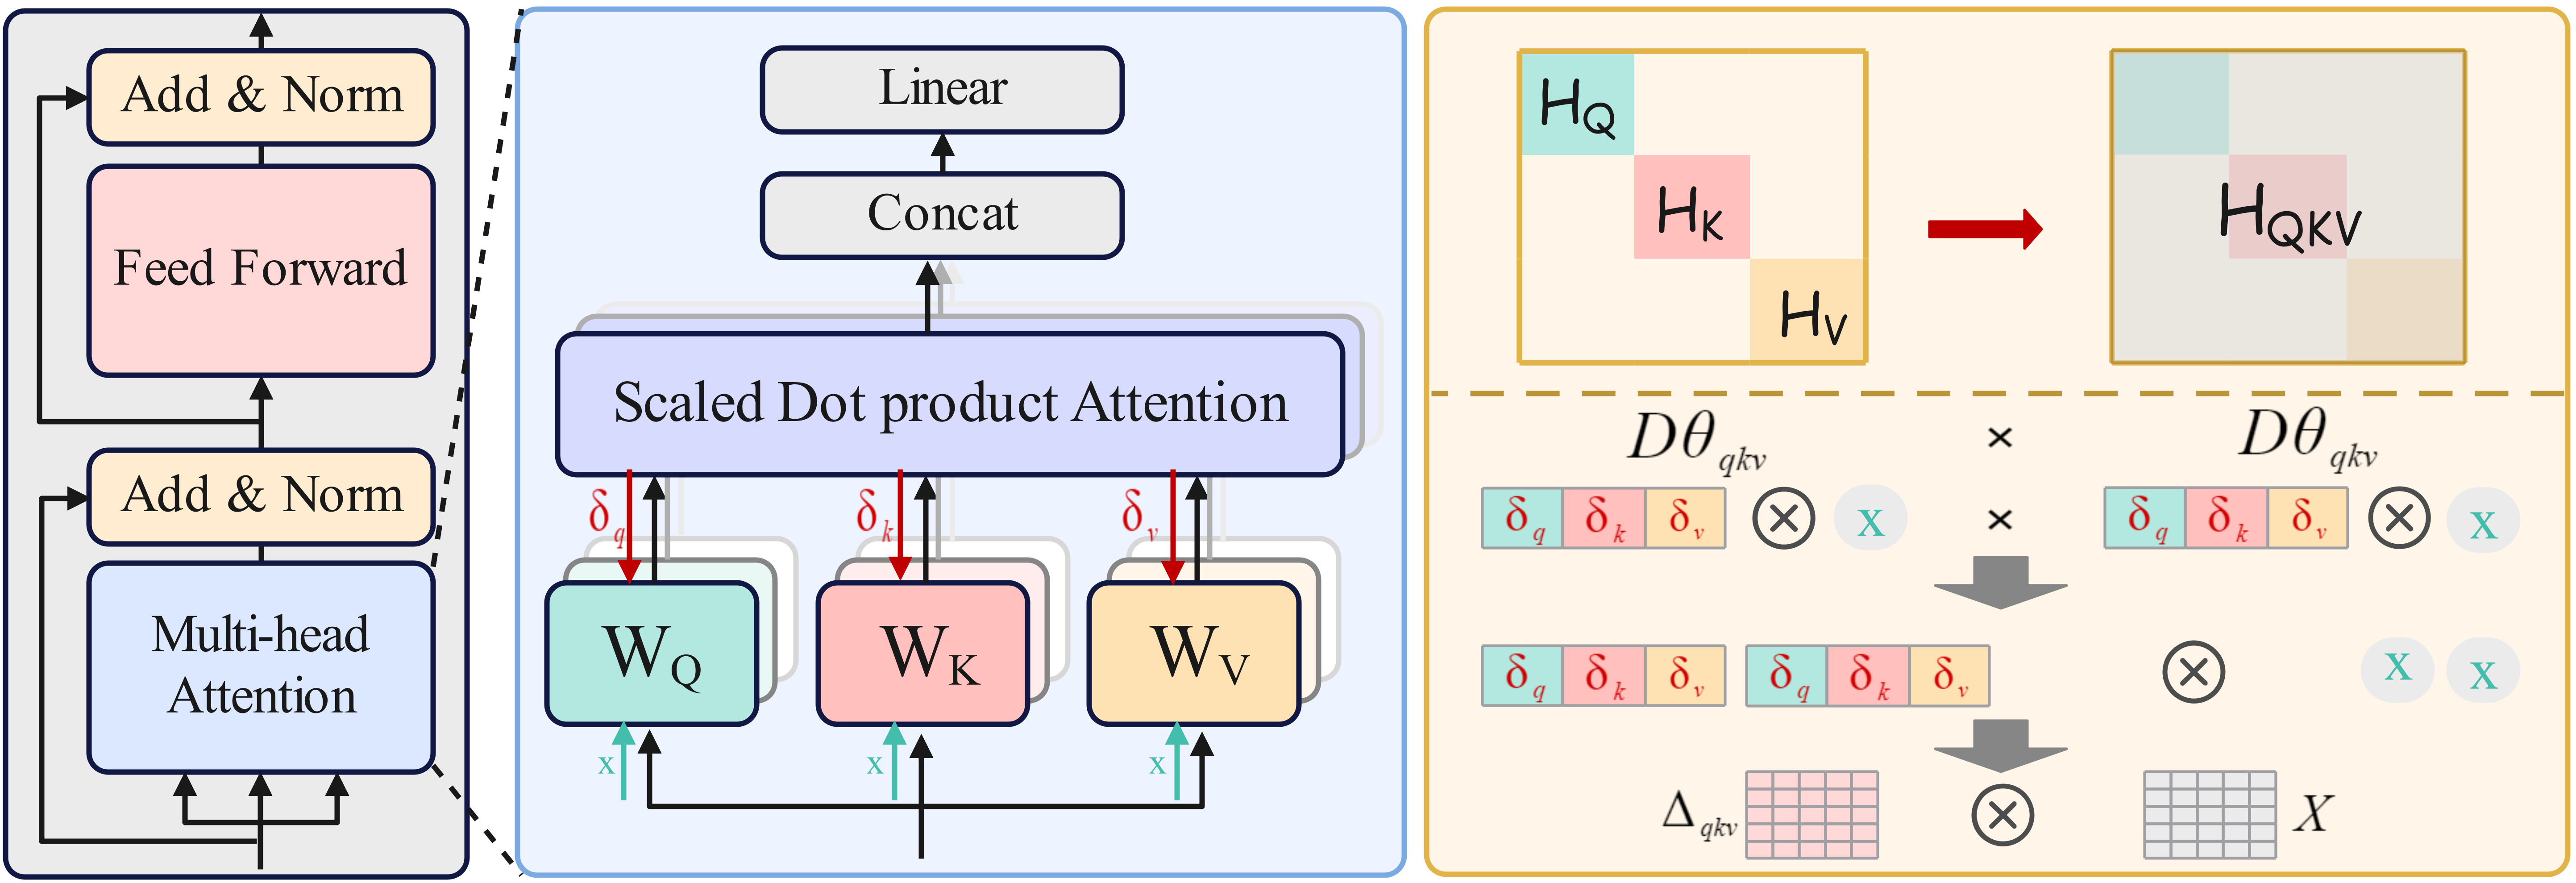
\includegraphics[width=1\textwidth]{multi-head-attention.png}
\end{center}
\caption{Kronecker Product in calculating iHVP}
\label{multi-head-attention}
\end{figure}

Then, as the right-lower corner of Figure~\ref{multi-head-attention} shows, by decomposing the Hessian matrix into a kronecker product of smaller matrices and computing the inverse of each smaller matrix, we can avoid directly inverting the entire Hessian matrix, significantly reducing computational cost, and accelerate this process:
%将海森矩阵分解为小矩阵的Kronecker积, 并对每个小矩阵计算逆矩阵, 避免了直接在整个海森矩阵上计算逆矩阵,极大地降低了计算开销.

\textbf{Forward propagation}:
\begin{equation}
    Attention(Q,K,V) = softmax(\frac{QK^{T}}{\sqrt{d_k}})V
\end{equation}

% zk:以下的公式符号可能需要讲解,如D_θ,Dθ_{Q/K/V}, DW_{Q/K/V}, D_{Q/K/V}, H_{qkv}, G_{qkv}, x, X是什么,或者说我们按照哪篇tutorial的setting进行计算?

\textbf{Backward propagation}:
\begin{equation}
    D\theta =vec(DW)=\delta\otimes x
\end{equation}
Here, $\otimes$ denotes the Kronecker product, and $vec()$ represents the vectorization operation. Thus, the gradient of $\theta_{qkv}$ can be written as:

\begin{equation}
    D\theta_{qkv} = \begin{bmatrix} \mathbf{vec(DW_Q)} \\ \mathbf{vec(DW_K)} \\ \mathbf{vec(DW_V)} \end{bmatrix} \\
 = \begin{bmatrix} \mathbf{\delta}_q \\ \mathbf{\delta}_k \\ \mathbf{\delta}_v \end{bmatrix} \otimes x
\end{equation}
Let $\delta_{qkv}$
 $= \begin{bmatrix} \mathbf{\delta}_q \\ \mathbf{\delta}_k \\ \mathbf{\delta}_v \end{bmatrix} $. Then, the Hessian matrix $H_{qkv}$ can be estimates by:
\begin{equation}
\begin{aligned}
    H_{qkv} = E(D\theta_{qkv} {D\theta_{qkv}}^T)=E(\delta_{qkv}\delta_{qkv}^T\otimes x_{qkv}x_{qkv}^T) \\
    \approx E(\delta_{qkv}\delta_{qkv}^T) \otimes E(x_{qkv}x_{qkv}^T) = \Delta_{qkv} \otimes X_{qkv}
\end{aligned}
\end{equation}

Also, $H_o = \Delta_o \otimes X_o$. Thus, the iHVP of the attention layer can be estimated as follows: 

\begin{equation}
\begin{aligned}
H_{att}^{-1}v_{att} = 
\begin{bmatrix}\mathbf {H_{qkv}^{-1}v_{qkv}} \\ \mathbf{H_o^{-1}v_o}  \end{bmatrix}
= \begin{bmatrix} \mathbf{(\Delta_{qkv} \otimes X_{qkv})^{-1}v_{qkv}} \\ \mathbf{(\Delta_{o} \otimes X_o)^{-1}v_o} \end{bmatrix} \\
= \begin{bmatrix} \mathbf{(\Delta_{qkv}^{-1} \otimes X_{qkv}^{-1})v_{qkv}} \\ \mathbf{(\Delta_{o}^{-1} \otimes X_o^{-1})v_o} \end{bmatrix}
= \begin{bmatrix} \mathbf{vec(\Delta_{qkv}^{-1} V_{qkv} X_{qkv}^{-1})} \\ \mathbf{vec(\Delta_{o}^{-1} V_o X_o^{-1})} \end{bmatrix}
\end{aligned}
\end{equation}
% \begin{center}
% $(G+\lambda I)^{-1}v = vec(Q_x^T[(Q_xVQ_{qkv}^T)\varnothing unvec(diag^{-1}(\Lambda+\lambda I))]Q_{qkv})$
% \end{center}
% $\varnothing$denotes element-wise division, and $unvec()$ represents the inverse operation of $vec()$, $Q_{qkv}$ and $Q_x$ are the eigenvalue decompositions of $E_{qkv}$ and $X$, respectively. $E_{qkv} = Q_{qkv}\Lambda_{qkv}Q_{qkv}^T$, $X = Q_x\Lambda_{x}Q_x^T$, $\Lambda_{ii} = E[((Q_{qkv} \otimes Q_S)D\theta)_i^2]$

where $v_{att}$, $v_{qkv}$, $v_{o}$ represent the gradient of reference dataset $D_r$ on parameters $\theta_{att}$, $\theta_{qkv}$, $\theta_{o}$, respectively. Thus, the influence score of attention layers can be written as:  $I_{\theta_{att}} = -\nabla L(\theta_{att}, z)H_{att}^{-1}v_{att}$.


To avoid the excessive memory usage of validation set gradients, we apply the Johnson-Lindenstrauss Lemma to reduce the dimensionality of both the iHVP computation results and the training data gradients $\nabla L(\theta,z)$.
\section{Experiment}

\subsection{Experiment Setup}

%%zhp(solved): 4.1这一节,不用拆那么多小节,省点空间,像rhos-1/mates那样写,一段话讲一下我们用什么预训练模型,预训练的参数(lr之类的);一段话讲一下用什么数据作为训练集和验证集,embedding用什么模型;一段话写baselines,一段话写评测细节。
\textbf{Dataset Preparation.}
We use the entire 627B-token SlimPajama dataset as the candidate pool $D_c$. In the clustering process, the BAAI/bge-large-en-v1.5 model is employed to generate embeddings for the input data, and approximately 600 million data points from the candidate pool $D_c$ are clustered into 10,000 groups using the $k$-means algorithm. We use LAMBADA ~\citep{paperno2016lambada} as our reference set $D_r$, which is a widely used language modeling task and often serves as a validation benchmark for language model pretraining. ~\citep{yu2024mates, xie2023data, hoffmann2022empirical}.


%%zhp: batchsize可以写出来了

\textbf{Experimental settings.}
We train a transformer-based decoder-only language model that contains 1.3B parameters, uses RoPE embeddings ~\citep{su2023enhanced}, and has a maximum context window of 1024 tokens ~\citep{touvron2023llama}. 
%
%Firstly, we randomly select 20B tokens from $D_c$ to train the model from scratch. 
Following the setting of MATES~\citep{su2023enhanced}, 30B tokens out of the 627B are selected for training using \texttt{Quad} and compare with baselines.
%
%high quality data from $D_c$ using \texttt{Quad} and com
%
%Then, we aim to select 10B tokens high quality data from $D_c$ using \texttt{Quad} and other baselines to train the model.
%, which is similar to the setting of data annealing~\citep{blakeney2024does}. 
The learning rate is set to $5 \times 10^{-5}$, the batch size is set to 4096, and the Adam optimizer is employed with hyperparameters $\beta_1 = 0.9, \beta_2 = 0.95, \epsilon = 10^{-8}$. As for Multi-Armed Badit, we set the $\alpha$ = 0.002 , sample proporation $\gamma$ = 0.05 and the sample threshold $\tau$ as 0.0025.

%%zhp: 这句话没看懂想表达什么,所有的baseline我们采10B tokens,是啥意思?
\textbf{Baselines.} We compare our methods with several baselines. (1) \texttt{Random} samples  data from the entire candidate dataset randomly. (2) \texttt{Qurating} uses the large language model to select data. (3) \texttt{DSIR} selects data instances that are similar to the LAMBADA dataset. (4) \texttt{PPL} uses perplexity-based data selection, $i.e.,$ selecting data instances with the lowest perplexity scores. (5) \texttt{MATES} trains a surrogate model to evaluate the influence of each data instance on the target model.

\textbf{Evaluation datasets.}
To comprehensively evaluate the capabilities of pretrained models, we conduct  experiments on various downstream tasks covering three significant categories:
%lambada主要由名著中的语料所构成,提升大模型的commonsense reasoning能力以及reading comprehension能力

General Knowledge: ARC-C, ARC-E~\citep{clark2018think}, and SciQ ~\citep{welbl2017crowdsourcing}.

Commonsense Reasoning: HellaSwag ~\citep{zellers2019hellaswag}, SIQA ~\citep{sap2019social}, WinoGrande~\citep{sakaguchi2021winogrande}, Logiqa ~\citep{liu2020logiqa}.

Reading Comprehension: OpenbookQA ~\citep{mihaylov2018can}, and BoolQ~\citep{clark2019boolq}.

Evaluations are conducted using the lm-evaluation-harness~\citep{gao10256836framework} framework  and the average accuracy ($i.e.,$ Overall Score) is reported for comparison.


%%zhp(solved): 实验这里写到二级小标题/小章节就好了,不要再拆三级标题,浪费空间又显得内容很少。

\subsection{Results}

\textbf{Overall Performance.}
As demonstrated in Table~\ref{table1}, our method surpasses all the baseline methods in downstream tasks with zero-shot evaluation. 
%We observe that almost all baselines show marginal improvement over random selection. 
%These results reveal the promising potential of our method in elevating the scaling law of foundation models.
To be specific, we can observe that on General Knowledge and Reading Comprehension tasks, \texttt{Quad} has the improvement of 1.75\% and 1.98\% respectively compared with \texttt{Random}.
\texttt{Quad} outperforms \texttt{DSIR} and \texttt{Semdedup} because they use rule-based heuristics to select data without considering the model. Although \texttt{PPL} and \texttt{MATES} consider the model, they do not perform well because the former one always selects some simple and duplicated instances, and the surrogate model of the latter one is small and lacking of enough training data.  \texttt{Qurating} generally performs the best among other baselines, but still worse than our approach, and it incorporates the highest FLOPS(1e19) because of the usage of LLMs for data selection.
 In terms of the FLOPs, we can observe that except the methods ($i.e.,$ \texttt{DSIR}, \texttt{SemDeDup}) that use simple heuristics, we consume minimal computation resources because our MAB solution samples from clusters without considering the entire candidate dataset like \texttt{PPL}, \texttt{Qurating} and \texttt{MATES}.
 
%同时,所消耗的flops仅次于DSIR、SemDeDup这些基于启发式规则的数据筛选方法
% Please add the following required packages to your document preamble:
% \usepackage[table,xcdraw]{xcolor}
% Beamer presentation requires \usepackage{colortbl} instead of \usepackage[table,xcdraw]{xcolor}


%%zhp(solved): 主表还是以表格+数字的形式展现出来吧,排版和格式啥的参考mates的table1吧

%\begin{figure}[h]
%\begin{center}
%\framebox[4.0in]{$\;$}
%\includegraphics[width=1\textwidth]{table1.png}
%\end{center}
%\caption{Overall Performance.}
%\end{figure}
\renewcommand{\arraystretch}{1.05} % 增加行间距
\begin{table}[t]
\caption{Overall Performance}
\begin{center}
\scalebox{0.9}{
\begin{tabular}{cccccc}
\toprule
\textbf{Selection Method} & \makecell{\textbf{General}\\ \textbf{Knowledge}\\ \textit{(3 tasks)}} & \makecell{\textbf{Commonsense}\\ \textbf{Reasoning}\\ \textit{(4 tasks)}} & \makecell{\textbf{Reading}\\ \textbf{Comprehension}\\ \textit{(2 tasks)}} & \textbf{Overall} & \textbf{FLOPs}  \\ \midrule
Random                                                        &          50.33         &           36.19            &            39.09           &    41.55  &7.66   \\ \midrule
DSIR                                               &        50.37\textsuperscript{\colorbox{green!15}{\textcolor{black}{$\uparrow$0.04}}}           &             34.01\textsuperscript{\colorbox{red!15}{\textcolor{black}{$\downarrow$2.18}}}          &             38.80\textsuperscript{\colorbox{red!15}{\textcolor{black}{$\downarrow$1.29}}}          &    40.53\textsuperscript{\colorbox{red!15}{\textcolor{black}{$\downarrow$1.02}}}    &7.66\\ 

PPL                                                          &          48.71\textsuperscript{\colorbox{red!15}{\textcolor{black}{$\downarrow$1.62}}}         &            \textbf{37.72\textsuperscript{\colorbox{green!15}{\textcolor{black}{$\uparrow$1.53}}}}           &            38.57\textsuperscript{\colorbox{red!15}{\textcolor{black}{$\downarrow$0.52}}}           &     41.57\textsuperscript{\colorbox{green!15}{\textcolor{black}{$\uparrow$0.02}}}  & 9.51  \\ 

Semdedup                                                         &         50.99\textsuperscript{\colorbox{green!15}{\textcolor{black}{$\uparrow$0.66}}}          &            36.11\textsuperscript{\colorbox{red!15}{\textcolor{black}{$\downarrow$0.08}}}           &            39.44\textsuperscript{\colorbox{green!15}{\textcolor{black}{$\uparrow$0.35}}}          &     41.81\textsuperscript{\colorbox{green!15}{\textcolor{black}{$\uparrow$0.26}}} & 8.11   \\ 

Qurating                                                      &           \underline{51.56}\textsuperscript{\colorbox{green!15}{\textcolor{black}{$\uparrow$1.23}}}        &           35.93\textsuperscript{\colorbox{red!15}{\textcolor{black}{$\downarrow$0.26}}}            &             39.70\textsuperscript{\colorbox{green!15}{\textcolor{black}{$\uparrow$0.61}}}          &    \underline{42.01}\textsuperscript{\colorbox{green!15}{\textcolor{black}{$\uparrow$0.46}}} &13.66   \\ 

MATES                                                         &     50.45\textsuperscript{\colorbox{green!15}{\textcolor{black}{$\uparrow$0.12}}}              &       36.06\textsuperscript{\colorbox{red!15}{\textcolor{black}{$\downarrow$0.13}}}                &      \underline{39.83}\textsuperscript{\colorbox{green!15}{\textcolor{black}{$\uparrow$0.74}}}                 &   41.93\textsuperscript{\colorbox{green!15}{\textcolor{black}{$\uparrow$0.38}}}    &9.81  \\ \midrule

Quad(ours)                                                          &         \textbf{52.08\textsuperscript{\colorbox{green!15}{\textcolor{black}{$\uparrow$1.75}}}}          &           \underline{37.03}\textsuperscript{\colorbox{green!15}{\textcolor{black}{$\uparrow$0.84}}}            &           \textbf{41.07\textsuperscript{\colorbox{green!15}{\textcolor{black}{$\uparrow$1.98}}}}            &     \textbf{42.94\textsuperscript{\colorbox{green!15}{\textcolor{black}{$\uparrow$1.39}}}} &9.15 \\ \bottomrule
\end{tabular}}

\end{center}
\label{table1}
\end{table}


%\subsubsection{effectiveness of clustering}
%In this section, we compare our method with those domain-based data selection methods. In our experiments, we found that even the most advanced domain-based data-mixing methods could not surpass the performance of simply selecting the top-k clusters based on influence scores. This indicates that clustering is a better approach for distinguishing data quality compared to the domain provided by SlimPajama.
% %在实验中我们可以发现,哪怕是最先进的基于domain的data-mixing方法,效果都无法超越按照influence score选择topk个簇的效果。可见,相比于slimpajama自带的domain,聚类是一种更好地用于区分数据质量的方式。
% \begin{table}[t]
% \caption{effectiveness of clustering}
% \label{sample-table}
% \begin{center}
% \scalebox{0.8}{
% \begin{tabular}{|c|c|c|c|c|}
% \hline
% {\color[HTML]{1D2129}} \textbf{Selection Method} & \begin{tabular}[c]{@{}c@{}}\textbf{General Knowledge}\\ (3 tasks)\end{tabular} & \begin{tabular}[c]{@{}c@{}}\textbf{Commonsense Reasoning}\\ (3 tasks)\end{tabular} & \begin{tabular}[c]{@{}c@{}}\textbf{Reading Comprehension}\\ (3 tasks) \end{tabular} & \textbf{overall} \\ \hline
% Random(30B tokens)                                                        &         50.33          &          31.26             &           43.06            &      41.55   \\ \hline
% DoReMi                                                         &          50.49         &             30.56          &           42.92            &     41.32    \\ \hline
% DOGE                                                      &                   &                       &                       &         \\ \hline
% Temperature                                                      &                   &                       &                       &         \\ \hline
% DMLaw                                               &                   &                       &                       &         \\ \hline
% topk                                               &                   &                       &                       &         \\ \hline
% \end{tabular}}
% \end{center}
% \end{table}

%%zhp(solved): 这里的标题跟方法中我们的模块名对齐,不要直接写MAB
%%zhp: 加一些分析和结论性的话
%%zhp: 这里就说我们对我们模块中的哪些参数做了消融,然后结果怎么样,也是要加一些分析和结论
\textbf{Effectiveness of MAB.}
This section evaluates the effectiveness of the MAB approach for data selection in contrast to the straightforward method of choosing the top-$k$ clusters with the highest influence scores for model training. To be specific, we randomly select an equivalent number of data points from the top 150, 500, and 1000 clusters.  Figure~\ref{experiment-fig1} illustrates the trade-off between data quality and diversity: clusters with higher influence scores do not necessarily enhance model performance on downstream evaluation sets because of their lack of diversity. Hence, the multi-armed bandit method can more effectively capture the trade-off between quality and diversity across clusters, resulting in  superior performance on downstream evaluation sets, as opposed to merely choosing the top-$k$ clusters.%从实验中可以看出,多臂老虎机可以更好地平衡簇与簇之间的探索与利用,在下游评测集中的表现远高于以簇为单位进行筛选
%替换为一张top150 top500 top1000 mab的图片

%\begin{table}[t]
%\caption{effectiveness of Multi-Armed Bandit}
%\label{sample-table}
%\begin{center}
%\scalebox{0.8}{
%\begin{tabular}{|c|c|c|c|c|}
%\hline
%{\color[HTML]{1D2129}} \textbf{Selection Method} & \begin{tabular}[c]{@{}c@{}}\textbf{General Knowledge}\\ (3 tasks)\end{tabular} & \begin{tabular}[c]{@{}c@{}}\textbf{Commonsense Reasoning}\\ (3 tasks)\end{tabular} & \begin{tabular}[c]{@{}c@{}}\textbf{Reading Comprehension}\\ (3 tasks) \end{tabular} & \textbf{overall} \\ \hline
%Random(30B tokens)                                                        &         50.33          &           31.26            &             43.06          &     41.55    \\ \hline
%top150 clusters                                                         &            49.50       &             32.39         &           44.24            &     42.04    \\ \hline
%top500 clusters                                                      &          50.66         &                32.11       &           44.66            &     42.47    \\ \hline
%top1000 clusters                                                      &          50.45         &               31.57       &            42.53           &     41.52    \\ \hline
%Multi-armed Bandit                                              &         52.08          &           32.01            &           44.74            &     42.94        \\ \hline

%\end{tabular}}
%\end{center}
%\end{table}

%%zhp: fig4和5的标题好好写一下吧,比如fig4里面的 (a) Effectiveness of ***,或者参考别人的论文,简单写两三句话介绍下


\begin{figure}
  \begin{minipage}[t]{0.25\linewidth}
    \centering
    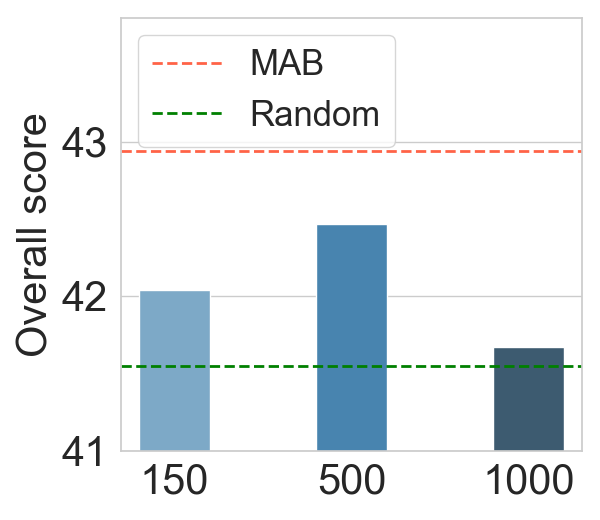
\includegraphics[scale=0.23]{exp-fig1.png}
    \subcaption{MAB vs. top-$k$ clusters}
    \label{experiment-fig1}
  \end{minipage}%
  \begin{minipage}[t]{0.25\linewidth}
    \centering
    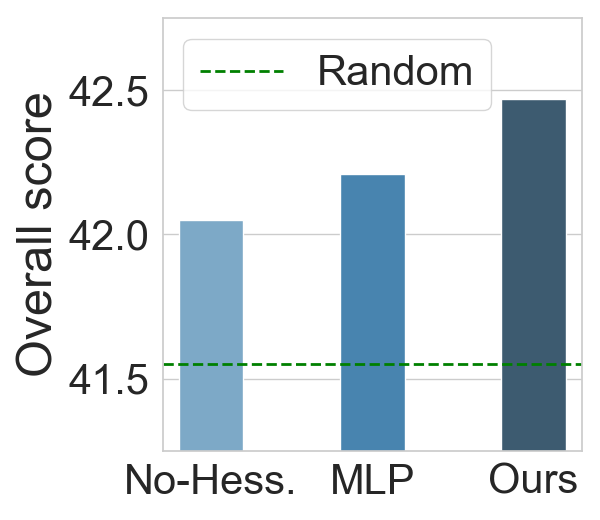
\includegraphics[scale=0.23]{exp-fig2.png}
    \subcaption{Influence accuracy}
    \label{experiment-fig2}
  \end{minipage}%
  \begin{minipage}[t]{0.25\linewidth}
    \centering
    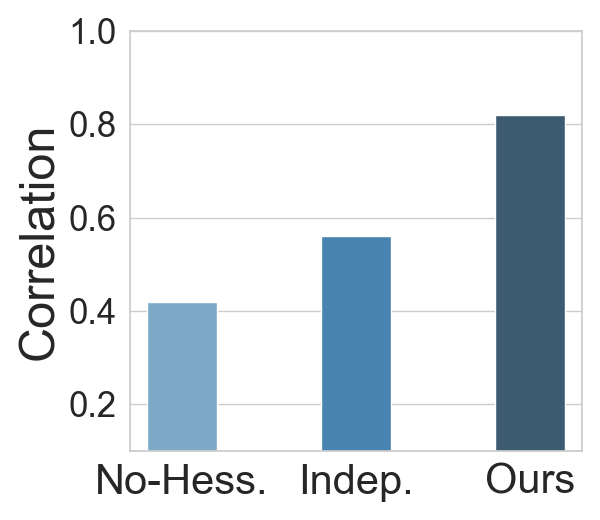
\includegraphics[scale=0.23]{exp-fig6.png}
    \subcaption{Influence correlation}
    \label{experiment-fig6}
  \end{minipage}%
  \begin{minipage}[t]{0.25\linewidth}
    \centering
    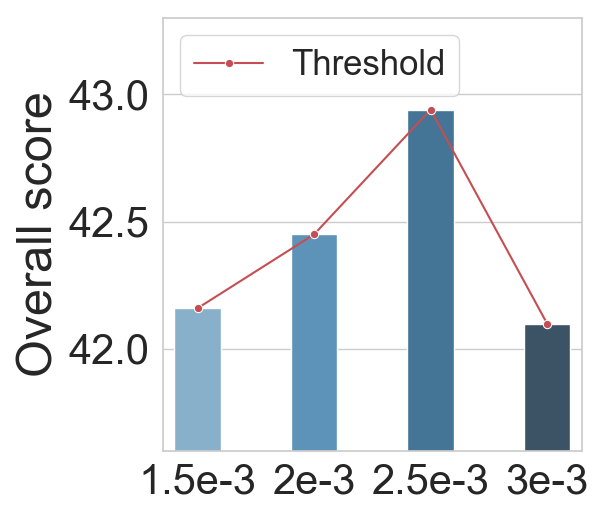
\includegraphics[scale=0.23]{exp-fig4.png}
    \subcaption{Sample threshold $\tau$}
    \label{experiment-fig4}
  \end{minipage}
  \caption{(a) shows the effectiveness of the MAB method; (b) shows the accuracy of calculating the influence function on MLP and attention layers; (c) shows the correlation between Query, Key, Value layers impact a lot on the accuracy of influence calculation; (d) shows the model performance of varying sample threshold $\tau$.}
  \label{fig:experiment2}
\end{figure}

\iffalse
\begin{figure}
  \begin{minipage}[t]{0.5\linewidth}
    \centering
    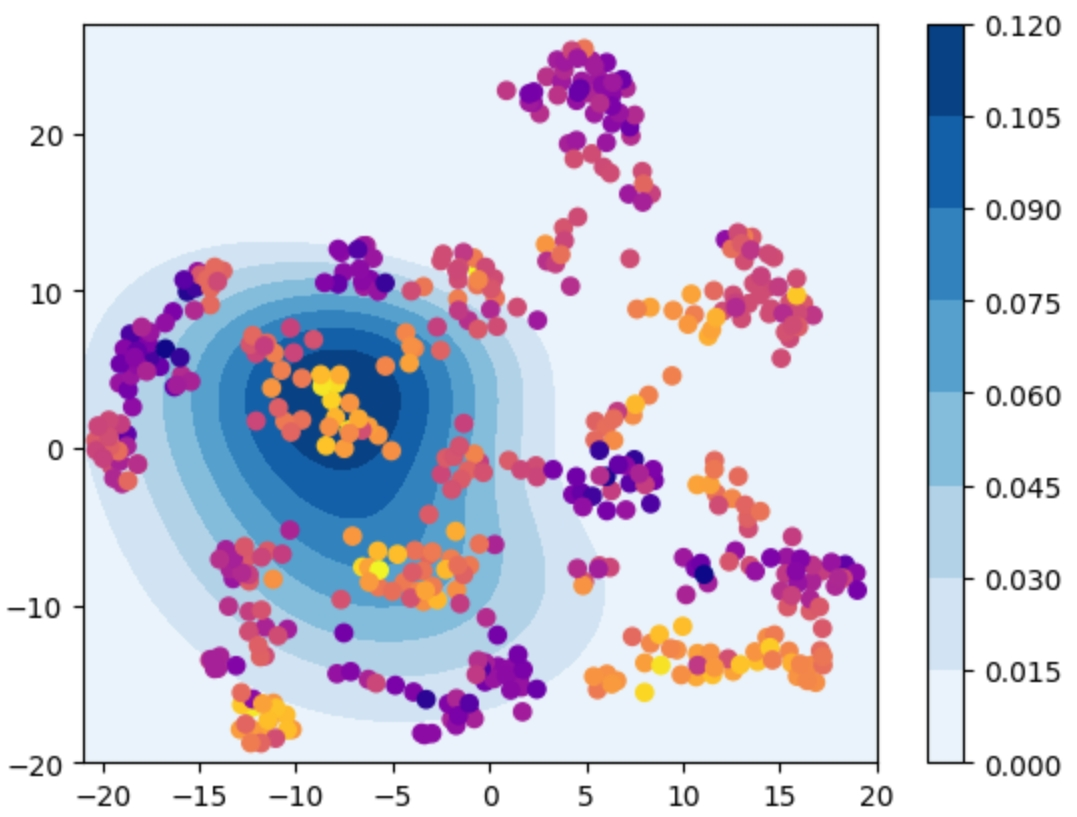
\includegraphics[scale=0.18]{demo-1.jpg}
    \subcaption{low exploration weight}
    \label{demo-1}
  \end{minipage}%
  \begin{minipage}[t]{0.65\linewidth}
    \centering
    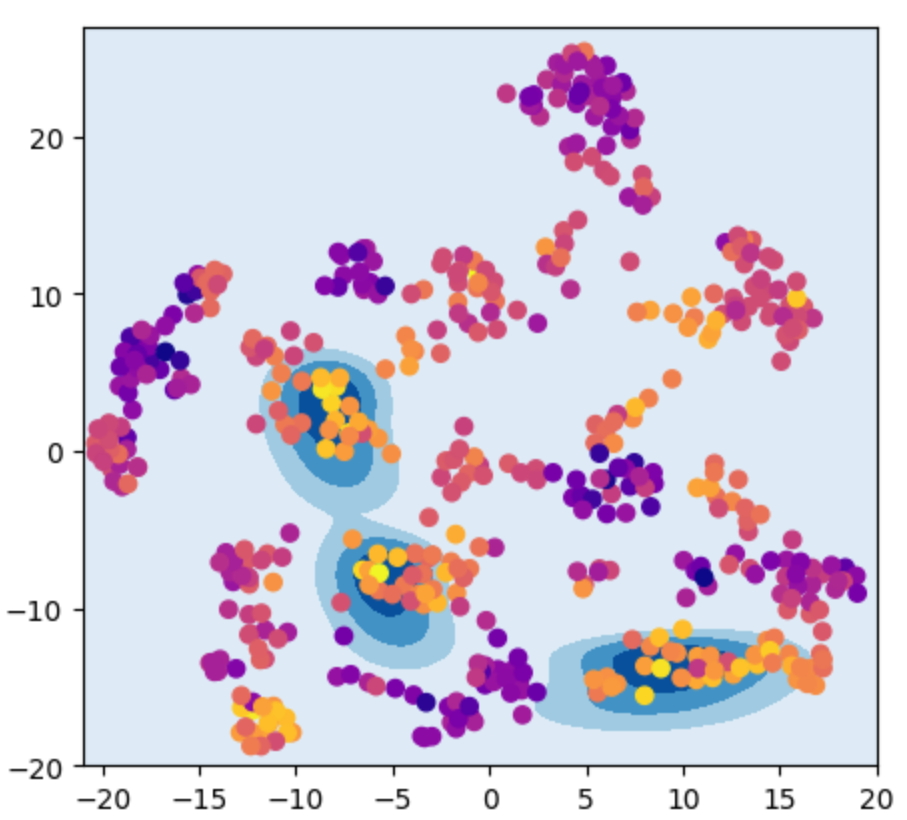
\includegraphics[scale=0.36]{demo-2.png}
    \subcaption{high selection threshold}
    \label{demo-2}
  \end{minipage}
  \caption{Demonstration of (a) demo-1 and (b) demo-2.}
  \label{fig:demo}
\end{figure}
\fi

%%zhp: 没有看到table4,另外论文这里的叫法,跟fig4的也不一致,这个肯定是要保持一致的

\textbf{Effectiveness of Influence Calculation.}
This experiment studies the effectiveness of our influence calculation method. In this section, we select the top 500 clusters with the highest scores using three methods: (1) \texttt{no-Hessian} ($i.e.,$ computing the gradient similarity between  training data and reference data~\citep{pruthi2020estimating}) without considering the Hessian matrix; (2)  \texttt{MLP}($i.e.,$ calculating influence function on MLP layers) and (3) \texttt{Ours} ($i.e.,$ calculating influence function on both MLP and attention layers).
%
From each cluster, we uniformly sample data to train the large model. As shown in Figure~\ref{experiment-fig2}, our solution (\texttt{MLP+Attention}) performs better than \texttt{MLP} because the attention layer considers more semantics. \texttt{no-Hessian} performs the worst because it does not precisely capture the impact of training data instances on the model without the Hessian matrix. 

Also, we conduct experiments to verify the relationship between the Query, Key, Value matrices, which is shown in Figure~\ref{experiment-fig6}.
%
In this experiment, we compare the Pearson correlation coefficients between the following three methods and the baseline approach, which computes the influence score for the attention layer without any acceleration. (1) \texttt{No-Hessian}($i.e.,$ computing the gradient similarity between  training data and reference data) without considering the Hessian matrix; (2) \texttt{Independent} ($i.e.,$ calculating the Hessian matrices of the query, key, and value layers independently) and (3) \texttt{Ours} ($i.e.,$ calculating the Hessian matrices of the query, key, and value layers as a whole).


%calculating the influence on the full set of parameters results in higher accuracy compared to calculating it only on the MLP layers. Moreover, the 2D-influence method, which incorporates the Hessian matrix, provides a better representation of the model's current state and captures the interaction information within the attention layers. As a result, it achieves a higher accuracy than the 1D-influence function computed on the full set of parameters.


%\begin{table}[t]
%\caption{effectiveness of EK-FAC influence function}
%\label{sample-table}
%\begin{center}
%\scalebox{0.8}{
%\begin{tabular}{|c|c|c|c|c|}
%\hline
%{\color[HTML]{1D2129}} \textbf{Selection Method} & \begin{tabular}[c]{@{}c@{}}\textbf{General Knowledge}\\ (3 tasks)\end{tabular} & \begin{tabular}[c]{@{}c@{}}\textbf{Commonsense Reasoning}\\ (3 tasks)\end{tabular} & \begin{tabular}[c]{@{}c@{}}\textbf{Reading Comprehension}\\ (3 tasks) \end{tabular} & \textbf{overall} \\ \hline
%Random                                                        &         50.33          &           31.26            &            43.06           &     41.55    \\ \hline
%\begin{tabular}[c]{@{}c@{}}\textbf{1D-influence function}\\ (mlp + attention layers)\end{tabular}                                                      &                 &                     &                       &        \\ \hline
%\begin{tabular}[c]{@{}c@{}}\textbf{2D-influence function}\\ (mlp layers)\end{tabular}                                                     &                   &                       &                       &         \\ \hline
%\begin{tabular}[c]{@{}c@{}}\textbf{2D-influence function}\\ (mlp + attention layers)\end{tabular}                                                &         50.66          &          32.11             &          44.66             &     42.47    \\ \hline
%\end{tabular}}
%\end{center}
%\end{table}

%%zhp(solved): 不用单独一章节来写ablation study,融入到4.2里面,4.2就一个overall performance,展示我们的效果,另外一个其实就是ablation study,展示我们方法各个模块以及超参对结果的影响,ablation study的效果对比可以通过具体数值和图表的形式。

%%zhp: 第五章写conclusion,主要就是写我们的总结以及我们的不足和未来的展望。
\subsection{Ablation Study}
This group of experiments performs ablation studies on the hyperparameters of \texttt{Quad}. Figure~\ref{experiment-fig4} and Figure~\ref{exploration} show the impact of sample threshold and $\alpha$ respectively.

%\textbf{Sample Data-size.}
%Figure~\ref{experiment-fig2} shows the impact of sample data-size.  If the sample size is small, In the early stage of the MAB, diversity is the primary focus.  If the sample data size is very large at this stage, exhausting the entire dataset too early makes it difficult to delve deeper into high-quality clusters, leading to lower overall data quality.  In the later stage, where exploiting the high-quality clusters becomes the focus, if the sample data size is too small, a disproportionate amount of sampling will occur in high-quality clusters, resulting in reduced data diversity.

\textbf{Sampling Threshold of Influence ($\tau$).}
 Setting the threshold too high or low will both degrade the model performance.  This is because the selected data instances tend to exist in few clusters with high influence scores, resulting in poor diversity. In contrast, when the threshold is set too low, the sampled instances will be from many clusters with low influence scores, which also degrades the model performance. %Overall, $XXX = 2.5e-3$ is an appropriate threshold.

%可以发现,无论sample threshold过高或过低,都会使得模型的性能下降

%我们可以发现,当采样的threshold较高时,所采的数据样本往往集中于高密度区域,从而导致数据的多样性较低,使得模型性能下降;当采样的threshold较低时,又会从诸多得分较低的簇中进行采样, 同样会使模型性能下降

%在这一部分中,我们探索保留infleunce值最低的阈值为多少时模型的效果最好;当threshold过低时,所筛选数据的;当threshold过高时,所筛选数据的多样性较差,对模型性能造成损伤
%\begin{table}[t]
%\caption{Sample Threshold}
%当sample threshold较低时,冗余的数据较多,从而导致多臂老虎机的采样;当sample threshod较高时,会导致数据多样性降低,从而导致最终的采
%\label{sample-table}
%\begin{center}
%\scalebox{0.8}{
%\begin{tabular}{|c|c|c|c|c|}
%\hline
%{\color[HTML]{1D2129}} \textbf{threshold} & \begin{tabular}[c]{@{}c@{}}\textbf{General Knowledge}\\ (3 tasks)\end{tabular} & \begin{tabular}[c]{@{}c@{}}\textbf{Commonsense Reasoning}\\ (3 tasks)\end{tabular} & \begin{tabular}[c]{@{}c@{}}\textbf{Reading Comprehension}\\ (3 tasks) \end{tabular} & \textbf{overall} \\ \hline
%0.0015                                                        &            49.50       &             32.39         &           44.24            &     42.04    \\ \hline
%0.002                                                        &           50.87       &             31.83        &           44.14            &     42.28    \\ \hline
%0.0025                                                      &        52.08           &           32.01            &        44.74               &     42.94    \\ \hline
%0.003                                                      &           50.59        &               31.69       &            43.56           &     41.95    \\ \hline
%\end{tabular}}
%\end{center}
%\end{table}


%\begin{table}[t]
%\caption{exploration \& exploitation}
%\label{sample-table}
%\begin{center}
%\scalebox{0.8}{
%\begin{tabular}{|c|c|c|c|c|}
%\hline
%{\color[HTML]{1D2129}} \textbf{Alpha} & \begin{tabular}[c]{@{}c@{}}\textbf{General Knowledge}\\ (3 tasks)\end{tabular} & \begin{tabular}[c]{@{}c@{}}\textbf{Commonsense Reasoning}\\ (3 tasks)\end{tabular} & \begin{tabular}[c]{@{}c@{}}\textbf{Reading Comprehension}\\ (3 tasks) \end{tabular} & \textbf{overall} \\ \hline
%0.001                                                      &        50.07           &           32.21           &            43.06           &     41.78    \\ \hline
%0.0025                                &        52.08           &           32.01            &        44.74               &     42.94    \\ \hline
%0.005                                                      &                   &                       &                       &         \\ \hline
%0.01                                                      &         50.22          &           31.13           &     44.36                  &     41.90    \\ \hline
%\end{tabular}}
%\end{center}
%\end{table}
\textbf{$\alpha$ for Quality-Diversity Balance.}
Our approach employs $\alpha$ to balance the diversity and quality in the MAB framework.  
%
When $\alpha$ is small, we tend to focus on the several clusters with high influence scores without considering diversity much, so the MAB framework is likely to get stuck in a local optimum. 
%
For example, this results in the model enhancing its performance in specific areas (such as Common Sense Reasoning in Figure~\ref{exploration} when $\alpha = 1.5e-3$), while the performance in other areas ($i.e.,$ General Knowledge and Reading Comprehension) is not good enough. Thus the overall score is not the optimal. 
%
However, when $\alpha$ is large, the MAB framework focuses too much on diversity without selecting enough high-quality data, which ultimately results in a limited improvement of model performance.

\begin{figure}[h]
\begin{center}
%\framebox[4.0in]{$\;$}
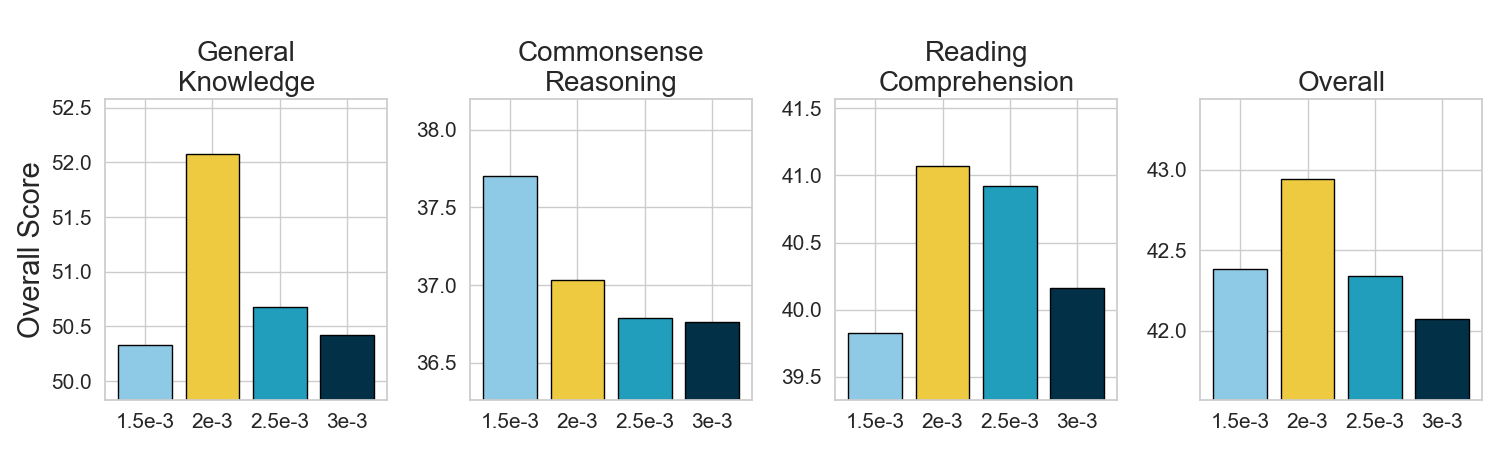
\includegraphics[width=1\textwidth]{exp-fig5.png}
\end{center}
\caption{$\alpha$ for Quality-Diversity Balance.}
\label{exploration}
\end{figure}
% \section{Limitation}
%尽管influence function是个非常强大的方法,但是其召回相关数据的能力很大程度上取决于模型本身的能力,因此,对于较小的1B模型,很难识别出具有复杂特征的数据。例如,判断一条数据是否与数学相关。


%%zhp: 少了conclusion章节。
\section{conclusion}
This paper presents \texttt{Quad}, a method designed to balance both the diversity and quality of data in pretraining data selection. \texttt{Quad} employs the influence function to identify data that benefits the model. First, we group the data into clusters and use a subset from each to represent the influence of the entire cluster. Given that influence scores within a cluster display some uncertainty, we view each cluster as an arm in an MAB framework. This method conducts samplings from high-quality clusters, allowing for more precise estimation of their influence scores and meanwhile maintaining the diversity. Moreover, we extend the influence function to attention layers and enhance the calculation efficiency to better measure the impact of data within each cluster on the model.

\bibliography{iclr2025_conference}
\bibliographystyle{iclr2025_conference}

\newpage
\appendix
\section{Appendix}

\begin{table}[h!]
\centering
\caption{Performance Comparison}
\scalebox{0.67}{
\begin{tabular}{lccccccccccccccc}
\toprule
\textbf{Selection Method}& \multicolumn{4}{c}{General Knowledge} & \multicolumn{5}{c}{Commonsense Reasoning} & \multicolumn{3}{c}{Reading Comprehension} & \textbf{Overall} \\
\cmidrule(lr){2-5} \cmidrule(lr){6-10} \cmidrule(lr){11-13} 
& arc-e & arc-c & sciq & \textbf{avg} & logiqa & hellaswag & siqa & winogrande & \textbf{avg} & openbookqa & boolq & \textbf{avg} & \\
\midrule
Random & 50.27 & 20.31 & 80.40 & \textbf{50.33} & 21.20 & 34.11 & 38.49 & 50.99 & \textbf{36.20} & 17.60 & 60.58 & \textbf{39.09} & \textbf{41.55} \\
Semdedup & 51.35 & 20.73 & 80.90 & \textbf{50.99} & 19.05 & 34.56 & 39.30 & 51.54 & \textbf{36.11} & 18.80 & 60.09 & \textbf{39.45} & \textbf{41.81} \\
MATES & 50.00 & 21.25 & 80.10 & \textbf{50.45} & 21.66 & 33.90 & 38.69 & 52.17 & \textbf{36.61} & 19.00 & 60.67 & \textbf{39.84} & \textbf{41.94} \\
PPL & 45.41 & 20.82 & 79.90 & \textbf{48.71} & 20.43 & 35.92 & 39.92 & 54.62 & \textbf{37.72} & 18.80 & 58.35 & \textbf{38.58} & \textbf{41.57} \\
DSIR & 49.28 & 20.14 & 81.70 & \textbf{50.37} & 21.20 & 30.89 & 35.98 & 47.99 & \textbf{34.02} & 16.20 & 61.41 & \textbf{38.81} & \textbf{40.53} \\
Qurating & 52.10 & 23.29 & 79.80 & \textbf{51.56} & 20.43 & 33.57 & 39.05 & 50.67 & \textbf{35.93} & 18.00 & 61.41 & \textbf{39.71} & \textbf{42.04} \\
Quad(ours) & 52.27 & 21.76 & 82.20 & \textbf{52.08} & 22.89 & 34.41 & 38.74 & 52.09 & \textbf{37.03} & 20.00 & 62.14 & \textbf{41.07} & \textbf{42.94} \\
\midrule
top$k$-cluster \\
top-150 & 48.61 & 20.90 & 79.00 & \textbf{49.50} & 23.66 & 34.51 & 39.00 & 51.78 & \textbf{37.24} & 19.20& 61.74 & \textbf{40.47} & \textbf{42.04} \\
top-500 & 51.05 & 21.25 & 79.70 & \textbf{50.67} & 22.73 & 34.40 & 39.20 & 52.41 & \textbf{37.19} & 18.80 & 62.76 & \textbf{40.78} & \textbf{42.48} \\
top-1000 & 49.96 & 20.99 & 80.40 & \textbf{50.45} & 21.97 & 34.00 & 38.74 & 50.2 & \textbf{36.23} & 18.20 & 60.61 & \textbf{39.41} & \textbf{41.67} \\
\bottomrule
\end{tabular}}
\end{table}




\begin{table}[h!]
\centering
\caption{Ablation Study of Threshold $\tau$}
\scalebox{0.7}{
\begin{tabular}{lccccccccccccccc}
\toprule
\textbf{Threshold}& \multicolumn{4}{c}{General Knowledge} & \multicolumn{5}{c}{Commonsense Reasoning} & \multicolumn{3}{c}{Reading Comprehension} & \textbf{Overall} \\
\cmidrule(lr){2-5} \cmidrule(lr){6-10} \cmidrule(lr){11-13} 
& arc-e & arc-c & sciq & \textbf{avg} & logiqa & hellaswag & siqa & winogrande & \textbf{avg} & openbookqa & boolq & \textbf{avg}  & \\
\midrule
0.0015     & 51.26 & 21.16 & 80.20 & \textbf{50.87} & 21.51 & 33.92 & 39.00 & 51.07 & \textbf{36.38} & 19.60 & 61.74 & \textbf{40.67} & \textbf{42.16} \\
0.0020     & 52.23 & 22.27 & 80.70 & \textbf{51.73} & 22.89 & 34.77 & 38.33 & 50.20 & \textbf{36.55} & 19.20 & 61.50 & \textbf{40.35} & \textbf{42.45} \\
0.0025    & 52.27 & 21.76 & 82.20 & \textbf{52.08} & 22.89 & 34.41 & 38.74 & 52.09 & \textbf{37.03} & 20.00 & 62.14 & \textbf{41.07} & \textbf{42.94} \\
0.0030     & 50.25 & 19.62 & 80.80 & \textbf{50.22} & 22.27 & 33.96 & 38.96 & 53.28 & \textbf{37.12} & 20.60 & 59.20 & \textbf{39.90} & \textbf{42.10} \\
\bottomrule
\end{tabular}}
\end{table}

\begin{table}[h!]
\centering
\caption{Ablation Study of $\alpha$}
\scalebox{0.73}{
\begin{tabular}{lccccccccccccccc}
\toprule
\textbf{Alpha} & \multicolumn{4}{c}{General Knowledge} & \multicolumn{5}{c}{Commonsense Reasoning} & \multicolumn{3}{c}{Reading Comprehension} & \textbf{Overall} \\
\cmidrule(lr){2-5} \cmidrule(lr){6-10} \cmidrule(lr){11-13}
& arc-e & arc-c & sciq & \textbf{avg} & logiqa & hellaswag & siqa & winogrande & \textbf{avg} & openbookqa & boolq & \textbf{avg} & \\
\midrule
0.0015 & 50.55 & 20.73 & 79.70 & \textbf{50.33} & 23.35 & 34.60 & 40.58 & 52.25 & \textbf{37.70} & 19.60 & 60.06 & \textbf{39.83} & \textbf{42.38} \\
0.0020 & 52.27 & 21.76 & 82.20 & \textbf{52.08} & 22.89 & 34.41 & 38.74 & 52.09 & \textbf{37.03} & 20.00 & 62.14 & \textbf{41.07} & \textbf{42.94} \\
0.0025 & 51.64 & 22.10 & 78.30 & \textbf{50.68} & 21.81 & 34.76 & 38.02 & 52.57 & \textbf{36.79} & 19.80 & 62.05 & \textbf{40.93} & \textbf{42.34} \\
0.0030 & 50.63 & 21.93 & 78.70 & \textbf{50.42} & 22.12 & 34.64 & 39.15 & 51.14 & \textbf{36.76} & 18.60 & 61.71 & \textbf{40.16} & \textbf{42.07} \\
\bottomrule
\end{tabular}}
\end{table}

\begin{table}[h!]
\centering
\caption{Effectiveness of Influence Calculation}
\scalebox{0.7}{
\begin{tabular}{lccccccccccccccc}
\toprule
\textbf{Method} & \multicolumn{4}{c}{General Knowledge} & \multicolumn{5}{c}{Commonsense Reasoning} & \multicolumn{3}{c}{Reading Comprehension} & \textbf{Overall} \\
\cmidrule(lr){2-5} \cmidrule(lr){6-10} \cmidrule(lr){11-13}
& arc-e & arc-c & sciq & \textbf{avg} & logiqa & hellaswag & siqa & winogrande & \textbf{avg} & openbookqa & boolq & \textbf{avg} & \\
\midrule
Random & 50.27 & 20.31 & 80.40 & \textbf{50.33} & 21.20 & 34.11 & 38.49 & 50.99 & \textbf{36.20} & 17.60 & 60.58 & \textbf{39.09} & \textbf{41.55} \\
No-Hessian & 49.03 & 20.99 & 80.50 & \textbf{50.20} & 22.58 & 33.40 & 38.89 & 52.41 & \textbf{36.82} & 19.20 & 61.50 & \textbf{40.35} & \textbf{42.06} \\
MLP & 50.63 & 21.50 & 78.90 & \textbf{50.34} & 22.89 & 33.32 & 38.74 & 52.57 & \textbf{36.88} & 19.60 & 61.77 & \textbf{40.69} & \textbf{42.21} \\
Ours & 51.05 & 21.25 & 79.70 & \textbf{50.67} & 22.73 & 34.40& 39.20 & 52.41 & \textbf{37.19} & 18.80 & 62.76 & \textbf{40.78} & \textbf{42.48} \\
\bottomrule
\end{tabular}}
\end{table}

\begin{table}[h!]
\centering
\caption{Model Architecture}
\begin{tabular}{ll}
\toprule
{\color[HTML]{1D2129} Hyperparameter} & Value               \\
\midrule
Vocabulary Size                       & 32,000              \\
MLP Ratio                             & 8/3                \\
Hidden Dimension Size                 & 2048                \\
Number of Layers                      & 24                  \\
Number of Attention Heads             & 16                  \\
Number of KV Attention Heads          & 16                  \\
RoPE Base                             & 10,000              \\
Maximum Context Window Length         & 1024                \\
Number of Parameters                  & 1,345,423,360(1.3B) \\
\bottomrule
\end{tabular}
\end{table}

% You may include other additional sections here.


\end{document}
